\documentclass[11pt]{article}\usepackage[]{graphicx}\usepackage[]{color}
%% maxwidth is the original width if it is less than linewidth
%% otherwise use linewidth (to make sure the graphics do not exceed the margin)
\makeatletter
\def\maxwidth{ %
  \ifdim\Gin@nat@width>\linewidth
    \linewidth
  \else
    \Gin@nat@width
  \fi
}
\makeatother

\definecolor{fgcolor}{rgb}{0.345, 0.345, 0.345}
\newcommand{\hlnum}[1]{\textcolor[rgb]{0.686,0.059,0.569}{#1}}%
\newcommand{\hlstr}[1]{\textcolor[rgb]{0.192,0.494,0.8}{#1}}%
\newcommand{\hlcom}[1]{\textcolor[rgb]{0.678,0.584,0.686}{\textit{#1}}}%
\newcommand{\hlopt}[1]{\textcolor[rgb]{0,0,0}{#1}}%
\newcommand{\hlstd}[1]{\textcolor[rgb]{0.345,0.345,0.345}{#1}}%
\newcommand{\hlkwa}[1]{\textcolor[rgb]{0.161,0.373,0.58}{\textbf{#1}}}%
\newcommand{\hlkwb}[1]{\textcolor[rgb]{0.69,0.353,0.396}{#1}}%
\newcommand{\hlkwc}[1]{\textcolor[rgb]{0.333,0.667,0.333}{#1}}%
\newcommand{\hlkwd}[1]{\textcolor[rgb]{0.737,0.353,0.396}{\textbf{#1}}}%
\let\hlipl\hlkwb

\usepackage{framed}
\makeatletter
\newenvironment{kframe}{%
 \def\at@end@of@kframe{}%
 \ifinner\ifhmode%
  \def\at@end@of@kframe{\end{minipage}}%
  \begin{minipage}{\columnwidth}%
 \fi\fi%
 \def\FrameCommand##1{\hskip\@totalleftmargin \hskip-\fboxsep
 \colorbox{shadecolor}{##1}\hskip-\fboxsep
     % There is no \\@totalrightmargin, so:
     \hskip-\linewidth \hskip-\@totalleftmargin \hskip\columnwidth}%
 \MakeFramed {\advance\hsize-\width
   \@totalleftmargin\z@ \linewidth\hsize
   \@setminipage}}%
 {\par\unskip\endMakeFramed%
 \at@end@of@kframe}
\makeatother

\definecolor{shadecolor}{rgb}{.97, .97, .97}
\definecolor{messagecolor}{rgb}{0, 0, 0}
\definecolor{warningcolor}{rgb}{1, 0, 1}
\definecolor{errorcolor}{rgb}{1, 0, 0}
\newenvironment{knitrout}{}{} % an empty environment to be redefined in TeX

\usepackage{alltt}

\usepackage{hyperref, lastpage, fancyhdr,multicol,caption,subcaption,tabularx}
\usepackage{amsmath,graphicx}
\usepackage{float}

\usepackage{geometry}
\usepackage{pdflscape}



\topmargin      -1.5cm   % read Lamport p.163
\oddsidemargin  -0.04cm  % read Lamport p.163
\evensidemargin -0.04cm  % same as oddsidemargin but for left-hand pages
\textwidth      16.59cm
\textheight     23.94cm
\parskip         7.2pt   % sets spacing between paragraphs
\parindent         0pt   % sets leading space for paragraphs
\pagestyle{empty}        % Uncomment if don't want page numbers
\pagestyle{fancyplain}

\usepackage{natbib} %need this for bibtex
\IfFileExists{upquote.sty}{\usepackage{upquote}}{}

\lhead{}
\chead{}
\rhead{}

\usepackage{setspace} %for double spacing
\doublespacing
\IfFileExists{upquote.sty}{\usepackage{upquote}}{}
\begin{document}




\begin{knitrout}
\definecolor{shadecolor}{rgb}{0.969, 0.969, 0.969}\color{fgcolor}\begin{kframe}
\begin{alltt}
\hlkwd{sum}\hlstd{(nhanes}\hlopt{$}\hlstd{modvigmin}\hlopt{==}\hlnum{0}\hlstd{)}\hlopt{/}\hlkwd{nrow}\hlstd{(nhanes)}
\end{alltt}
\begin{verbatim}
## [1] 0.07841659
\end{verbatim}
\begin{alltt}
\hlkwd{sum}\hlstd{(nhanes}\hlopt{$}\hlstd{vigmin}\hlopt{==}\hlnum{0}\hlstd{)}\hlopt{/}\hlkwd{nrow}\hlstd{(nhanes)}
\end{alltt}
\begin{verbatim}
## [1] 0.8801602
\end{verbatim}
\begin{alltt}
\hlkwd{sum}\hlstd{(nhanes}\hlopt{$}\hlstd{lightmin}\hlopt{==}\hlnum{0}\hlstd{)}\hlopt{/}\hlkwd{nrow}\hlstd{(nhanes)}
\end{alltt}
\begin{verbatim}
## [1] 0
\end{verbatim}
\end{kframe}
\end{knitrout}

\begin{knitrout}
\definecolor{shadecolor}{rgb}{0.969, 0.969, 0.969}\color{fgcolor}\begin{kframe}
\begin{alltt}
\hlcom{#no diff in modmin by day really except 7th}
\hlstd{nhanes} \hlopt \hlkwd{group_by}\hlstd{(rep)} \hlopt \hlkwd{summarise}\hlstd{(}\hlkwc{m}\hlstd{=}\hlkwd{mean}\hlstd{(modvigmin),}\hlkwc{s}\hlstd{=}\hlkwd{sd}\hlstd{(modmin)}\hlopt{/}\hlkwd{sqrt}\hlstd{(}\hlkwd{length}\hlstd{(modmin)))}
\end{alltt}
\begin{verbatim}
## # A tibble: 7 � 3
##     rep        m         s
##   <int>    <dbl>     <dbl>
## 1     1 22.60066 0.3411052
## 2     2 23.01777 0.3518468
## 3     3 22.96771 0.3583861
## 4     4 22.41386 0.3488521
## 5     5 22.24356 0.3589189
## 6     6 21.15523 0.3571320
## 7     7 19.41996 0.3616865
\end{verbatim}
\begin{alltt}
\hlcom{#no diff in modmin by day really except 7th and 2nd}
\hlstd{nhanes} \hlopt \hlkwd{group_by}\hlstd{(rep)} \hlopt \hlkwd{summarise}\hlstd{(}\hlkwc{m}\hlstd{=}\hlkwd{mean}\hlstd{(lightmin),}\hlkwc{s}\hlstd{=}\hlkwd{sd}\hlstd{(lightmin)}\hlopt{/}\hlkwd{sqrt}\hlstd{(}\hlkwd{length}\hlstd{(lightmin)))}
\end{alltt}
\begin{verbatim}
## # A tibble: 7 � 3
##     rep        m        s
##   <int>    <dbl>    <dbl>
## 1     1 258.6827 1.048918
## 2     2 261.5339 1.093391
## 3     3 258.6147 1.096388
## 4     4 258.8213 1.136550
## 5     5 258.2212 1.160056
## 6     6 255.2295 1.186014
## 7     7 244.4119 1.253172
\end{verbatim}
\begin{alltt}
\hlcom{#mondays most vig, fri-sun least, tues-thurs similar}
\hlstd{nhanes} \hlopt \hlkwd{group_by}\hlstd{(rep)} \hlopt \hlkwd{summarise}\hlstd{(}\hlkwc{m}\hlstd{=}\hlkwd{mean}\hlstd{(vigmin),}\hlkwc{s}\hlstd{=}\hlkwd{sd}\hlstd{(vigmin)}\hlopt{/}\hlkwd{sqrt}\hlstd{(}\hlkwd{length}\hlstd{(lightmin)))}
\end{alltt}
\begin{verbatim}
## # A tibble: 7 � 3
##     rep         m          s
##   <int>     <dbl>      <dbl>
## 1     1 0.9411853 0.06110670
## 2     2 0.8115414 0.05276647
## 3     3 0.8965840 0.06021138
## 4     4 0.7660865 0.05689883
## 5     5 0.7392597 0.05397894
## 6     6 0.8310108 0.06361269
## 7     7 0.6902050 0.06106663
\end{verbatim}
\begin{alltt}
\hlkwd{anova}\hlstd{(}\hlkwd{lm}\hlstd{(modvigmin}\hlopt{~}\hlkwd{as.factor}\hlstd{(rep),}\hlkwc{data}\hlstd{=}\hlkwd{subset}\hlstd{(nhanes,rep}\hlopt{<}\hlnum{6}\hlstd{)))} \hlcom{#first 5 days are similar, last two}
\end{alltt}
\begin{verbatim}
## Analysis of Variance Table
## 
## Response: modvigmin
##                   Df   Sum Sq Mean Sq F value Pr(>F)
## as.factor(rep)     4     2902  725.44  0.8288 0.5065
## Residuals      31937 27954416  875.30
\end{verbatim}
\end{kframe}
\end{knitrout}

\begin{knitrout}
\definecolor{shadecolor}{rgb}{0.969, 0.969, 0.969}\color{fgcolor}\begin{kframe}
\begin{alltt}
\hlcom{#weekends lower}
\hlstd{nhanes} \hlopt \hlkwd{group_by}\hlstd{(dow)} \hlopt \hlkwd{summarise}\hlstd{(}\hlkwc{m}\hlstd{=}\hlkwd{mean}\hlstd{(modvigmin),}\hlkwc{s}\hlstd{=}\hlkwd{sd}\hlstd{(modvigmin)}\hlopt{/}\hlkwd{sqrt}\hlstd{(}\hlkwd{length}\hlstd{(modvigmin)))}
\end{alltt}
\begin{verbatim}
## # A tibble: 7 � 3
##     dow        m         s
##   <int>    <dbl>     <dbl>
## 1     1 17.46672 0.3539009
## 2     2 23.63394 0.3753241
## 3     3 23.49455 0.3683897
## 4     4 23.63173 0.3842220
## 5     5 23.18340 0.3712310
## 6     6 22.43408 0.3639320
## 7     7 19.52794 0.3799264
\end{verbatim}
\begin{alltt}
\hlcom{#weekends and thursday lower, friday higher}
\hlstd{nhanes} \hlopt \hlkwd{group_by}\hlstd{(dow)} \hlopt \hlkwd{summarise}\hlstd{(}\hlkwc{m}\hlstd{=}\hlkwd{mean}\hlstd{(lightmin),}\hlkwc{s}\hlstd{=}\hlkwd{sd}\hlstd{(lightmin)}\hlopt{/}\hlkwd{sqrt}\hlstd{(}\hlkwd{length}\hlstd{(lightmin)))}
\end{alltt}
\begin{verbatim}
## # A tibble: 7 � 3
##     dow        m        s
##   <int>    <dbl>    <dbl>
## 1     1 239.7397 1.171315
## 2     2 259.8399 1.106457
## 3     3 260.0095 1.095333
## 4     4 259.8370 1.102353
## 5     5 256.6507 1.103868
## 6     6 263.0100 1.146749
## 7     7 256.8055 1.218114
\end{verbatim}
\begin{alltt}
\hlcom{#first day vig}
\hlstd{nhanes} \hlopt \hlkwd{group_by}\hlstd{(dow)} \hlopt \hlkwd{summarise}\hlstd{(}\hlkwc{m}\hlstd{=}\hlkwd{mean}\hlstd{(vigmin),}\hlkwc{s}\hlstd{=}\hlkwd{sd}\hlstd{(vigmin)}\hlopt{/}\hlkwd{sqrt}\hlstd{(}\hlkwd{length}\hlstd{(lightmin)))}
\end{alltt}
\begin{verbatim}
## # A tibble: 7 � 3
##     dow         m          s
##   <int>     <dbl>      <dbl>
## 1     1 0.7239862 0.06502960
## 2     2 0.9462687 0.06184397
## 3     3 0.8742129 0.05357820
## 4     4 0.8859250 0.06278267
## 5     5 0.8446359 0.05683506
## 6     6 0.7264334 0.05487292
## 7     7 0.6707994 0.05419137
\end{verbatim}
\begin{alltt}
\hlkwd{anova}\hlstd{(}\hlkwd{lm}\hlstd{(modvigmin}\hlopt{~}\hlkwd{as.factor}\hlstd{(dow),}\hlkwc{data}\hlstd{=}\hlkwd{subset}\hlstd{(nhanes,dow}\hlopt\hlkwd{c}\hlstd{(}\hlnum{2}\hlopt{:}\hlnum{6}\hlstd{))))} \hlcom{#M-F similar}
\end{alltt}
\begin{verbatim}
## Analysis of Variance Table
## 
## Response: modvigmin
##                   Df   Sum Sq Mean Sq F value Pr(>F)
## as.factor(dow)     4     6363 1590.75  1.7992 0.1259
## Residuals      31803 28118692  884.15
\end{verbatim}
\end{kframe}
\end{knitrout}


\begin{knitrout}
\definecolor{shadecolor}{rgb}{0.969, 0.969, 0.969}\color{fgcolor}\begin{kframe}
\begin{alltt}
\hlcom{#test for weekend effects}
\hlkwd{anova}\hlstd{(}\hlkwd{lm}\hlstd{(modvigmin} \hlopt{~} \hlkwd{as.factor}\hlstd{(weekend),}\hlkwc{data}\hlstd{=nhanes))}
\end{alltt}
\begin{verbatim}
## Analysis of Variance Table
## 
## Response: modvigmin
##                       Df   Sum Sq Mean Sq F value    Pr(>F)    
## as.factor(weekend)     1   181096  181096  214.83 < 2.2e-16 ***
## Residuals          42438 35773439     843                      
## ---
## Signif. codes:  0 '***' 0.001 '**' 0.01 '*' 0.05 '.' 0.1 ' ' 1
\end{verbatim}
\begin{alltt}
\hlkwd{anova}\hlstd{(}\hlkwd{lm}\hlstd{(lightmin} \hlopt{~} \hlkwd{as.factor}\hlstd{(weekend),}\hlkwc{data}\hlstd{=nhanes))}
\end{alltt}
\begin{verbatim}
## Analysis of Variance Table
## 
## Response: lightmin
##                       Df    Sum Sq Mean Sq F value    Pr(>F)    
## as.factor(weekend)     1   1042016 1042016  133.48 < 2.2e-16 ***
## Residuals          42438 331295573    7807                      
## ---
## Signif. codes:  0 '***' 0.001 '**' 0.01 '*' 0.05 '.' 0.1 ' ' 1
\end{verbatim}
\begin{alltt}
\hlkwd{anova}\hlstd{(}\hlkwd{lm}\hlstd{(vigmin} \hlopt{~} \hlkwd{as.factor}\hlstd{(weekend),}\hlkwc{data}\hlstd{=nhanes))}
\end{alltt}
\begin{verbatim}
## Analysis of Variance Table
## 
## Response: vigmin
##                       Df Sum Sq Mean Sq F value  Pr(>F)   
## as.factor(weekend)     1    202 202.477   9.714 0.00183 **
## Residuals          42438 884572  20.844                   
## ---
## Signif. codes:  0 '***' 0.001 '**' 0.01 '*' 0.05 '.' 0.1 ' ' 1
\end{verbatim}
\end{kframe}
\end{knitrout}

\begin{knitrout}
\definecolor{shadecolor}{rgb}{0.969, 0.969, 0.969}\color{fgcolor}\begin{kframe}
\begin{alltt}
\hlstd{nrep} \hlkwb{<-} \hlstd{(nhanes} \hlopt \hlkwd{group_by}\hlstd{(id)} \hlopt \hlkwd{summarise}\hlstd{(}\hlkwc{n}\hlstd{=}\hlkwd{length}\hlstd{(id)))}\hlopt{$}\hlstd{n}

\hlcom{#m1 <- lme(modvigmin~1,data=nhanes,random=~1|id,correlation=corAR1(form=~1|id),method="ML")}
\hlstd{m1} \hlkwb{<-} \hlkwd{lme}\hlstd{(modvigmin}\hlopt{~}\hlkwd{as.factor}\hlstd{(rep)}\hlopt{+}\hlkwd{as.factor}\hlstd{(dow),}\hlkwc{data}\hlstd{=nhanes,}\hlkwc{random}\hlstd{=}\hlopt{~}\hlnum{1}\hlopt{|}\hlstd{id,}\hlkwc{method}\hlstd{=}\hlstr{"ML"}\hlstd{)}

\hlstd{re} \hlkwb{<-} \hlkwd{rep}\hlstd{(}\hlkwd{unlist}\hlstd{(}\hlkwd{ranef}\hlstd{(m1)),nrep)}
\hlstd{nhanes}\hlopt{$}\hlstd{error} \hlkwb{<-} \hlstd{nhanes}\hlopt{$}\hlstd{modvigmin}  \hlopt{-} \hlkwd{predict}\hlstd{(m1)}
\hlstd{eht} \hlkwb{<-} \hlstd{nhanes} \hlopt \hlkwd{group_by}\hlstd{(id)} \hlopt \hlkwd{summarise}\hlstd{(}\hlkwc{e1}\hlstd{=error[}\hlnum{1}\hlstd{],}\hlkwc{e2}\hlstd{=error[}\hlnum{2}\hlstd{],}\hlkwc{e3}\hlstd{=error[}\hlnum{3}\hlstd{],}\hlkwc{e4}\hlstd{=error[}\hlnum{4}\hlstd{],}\hlkwc{e5}\hlstd{=error[}\hlnum{5}\hlstd{],}\hlkwc{e6}\hlstd{=error[}\hlnum{6}\hlstd{],}\hlkwc{e7}\hlstd{=error[}\hlnum{7}\hlstd{])}

\hlcom{# ind <- which(!is.na(eht$e7))}
\hlcom{# boxtest <- rep(0,length(ind))}
\hlcom{# for(i in 1:length(ind))\{}
\hlcom{#   boxtest[i] <- Box.test(unlist(eht[ind[i],-1]),lag=2,type="Ljung-Box")$p.value}
\hlcom{# \}}
\hlcom{# summary(boxtest)}

\hlcom{#lag 1 difference}
\hlstd{o1a} \hlkwb{=} \hlkwd{c}\hlstd{(eht}\hlopt{$}\hlstd{e1[nrep} \hlopt{>} \hlnum{1}\hlstd{],eht}\hlopt{$}\hlstd{e2[nrep} \hlopt{>} \hlnum{2}\hlstd{],eht}\hlopt{$}\hlstd{e3[nrep} \hlopt{>} \hlnum{3}\hlstd{],eht}\hlopt{$}\hlstd{e4[nrep} \hlopt{>} \hlnum{4}\hlstd{],eht}\hlopt{$}\hlstd{e5[nrep} \hlopt{>} \hlnum{5}\hlstd{],eht}\hlopt{$}\hlstd{e6[nrep} \hlopt{>} \hlnum{6}\hlstd{])}
\hlstd{o1b} \hlkwb{=} \hlkwd{c}\hlstd{(eht}\hlopt{$}\hlstd{e2[nrep} \hlopt{>} \hlnum{1}\hlstd{],eht}\hlopt{$}\hlstd{e3[nrep} \hlopt{>} \hlnum{2}\hlstd{],eht}\hlopt{$}\hlstd{e4[nrep} \hlopt{>} \hlnum{3}\hlstd{],eht}\hlopt{$}\hlstd{e5[nrep} \hlopt{>} \hlnum{4}\hlstd{],eht}\hlopt{$}\hlstd{e6[nrep} \hlopt{>} \hlnum{5}\hlstd{],eht}\hlopt{$}\hlstd{e7[nrep} \hlopt{>} \hlnum{6}\hlstd{])}
\hlkwd{cor}\hlstd{(o1a,o1b)}
\end{alltt}
\begin{verbatim}
## [1] -0.1000537
\end{verbatim}
\begin{alltt}
\hlcom{#lag 2 diff}
\hlstd{o2a} \hlkwb{=} \hlkwd{c}\hlstd{(eht}\hlopt{$}\hlstd{e1[nrep} \hlopt{>} \hlnum{2}\hlstd{],eht}\hlopt{$}\hlstd{e2[nrep} \hlopt{>} \hlnum{3}\hlstd{],eht}\hlopt{$}\hlstd{e3[nrep} \hlopt{>} \hlnum{4}\hlstd{],eht}\hlopt{$}\hlstd{e4[nrep} \hlopt{>} \hlnum{5}\hlstd{],eht}\hlopt{$}\hlstd{e5[nrep} \hlopt{>} \hlnum{6}\hlstd{])}
\hlstd{o2b} \hlkwb{=} \hlkwd{c}\hlstd{(eht}\hlopt{$}\hlstd{e3[nrep} \hlopt{>} \hlnum{2}\hlstd{],eht}\hlopt{$}\hlstd{e4[nrep} \hlopt{>} \hlnum{3}\hlstd{],eht}\hlopt{$}\hlstd{e5[nrep} \hlopt{>} \hlnum{4}\hlstd{],eht}\hlopt{$}\hlstd{e6[nrep} \hlopt{>} \hlnum{5}\hlstd{],eht}\hlopt{$}\hlstd{e7[nrep} \hlopt{>} \hlnum{6}\hlstd{])}
\hlkwd{cor}\hlstd{(o2a,o2b)}
\end{alltt}
\begin{verbatim}
## [1] -0.1892647
\end{verbatim}
\begin{alltt}
\hlcom{#lag 3 diff  }
\hlstd{o3a} \hlkwb{=} \hlkwd{c}\hlstd{(eht}\hlopt{$}\hlstd{e1[nrep} \hlopt{>} \hlnum{3}\hlstd{],eht}\hlopt{$}\hlstd{e2[nrep} \hlopt{>} \hlnum{4}\hlstd{],eht}\hlopt{$}\hlstd{e3[nrep} \hlopt{>} \hlnum{5}\hlstd{],eht}\hlopt{$}\hlstd{e4[nrep} \hlopt{>} \hlnum{6}\hlstd{])}
\hlstd{o3b} \hlkwb{=} \hlkwd{c}\hlstd{(eht}\hlopt{$}\hlstd{e4[nrep} \hlopt{>} \hlnum{3}\hlstd{],eht}\hlopt{$}\hlstd{e5[nrep} \hlopt{>} \hlnum{4}\hlstd{],eht}\hlopt{$}\hlstd{e6[nrep} \hlopt{>} \hlnum{5}\hlstd{],eht}\hlopt{$}\hlstd{e7[nrep} \hlopt{>} \hlnum{6}\hlstd{])}
\hlkwd{cor}\hlstd{(o3a,o3b)}
\end{alltt}
\begin{verbatim}
## [1] -0.2558842
\end{verbatim}
\begin{alltt}
\hlcom{#lag 4 diff}
\hlstd{o4a} \hlkwb{=} \hlkwd{c}\hlstd{(eht}\hlopt{$}\hlstd{e1[nrep} \hlopt{>} \hlnum{4}\hlstd{],eht}\hlopt{$}\hlstd{e2[nrep} \hlopt{>} \hlnum{5}\hlstd{],eht}\hlopt{$}\hlstd{e3[nrep} \hlopt{>} \hlnum{6}\hlstd{])}
\hlstd{o4b} \hlkwb{=} \hlkwd{c}\hlstd{(eht}\hlopt{$}\hlstd{e5[nrep} \hlopt{>} \hlnum{4}\hlstd{],eht}\hlopt{$}\hlstd{e6[nrep} \hlopt{>} \hlnum{5}\hlstd{],eht}\hlopt{$}\hlstd{e7[nrep} \hlopt{>} \hlnum{6}\hlstd{])}
\hlkwd{cor}\hlstd{(o4a,o4b)}
\end{alltt}
\begin{verbatim}
## [1] -0.2653008
\end{verbatim}
\begin{alltt}
\hlcom{#lag 5 diff}
\hlstd{o5a} \hlkwb{=} \hlkwd{c}\hlstd{(eht}\hlopt{$}\hlstd{e1[nrep} \hlopt{>} \hlnum{5}\hlstd{],eht}\hlopt{$}\hlstd{e2[nrep} \hlopt{>} \hlnum{6}\hlstd{])}
\hlstd{o5b} \hlkwb{=} \hlkwd{c}\hlstd{(eht}\hlopt{$}\hlstd{e6[nrep} \hlopt{>} \hlnum{5}\hlstd{],eht}\hlopt{$}\hlstd{e7[nrep} \hlopt{>} \hlnum{6}\hlstd{])}
\hlkwd{cor}\hlstd{(o5a,o5b)}
\end{alltt}
\begin{verbatim}
## [1] -0.1862721
\end{verbatim}
\end{kframe}
\end{knitrout}


\begin{knitrout}
\definecolor{shadecolor}{rgb}{0.969, 0.969, 0.969}\color{fgcolor}
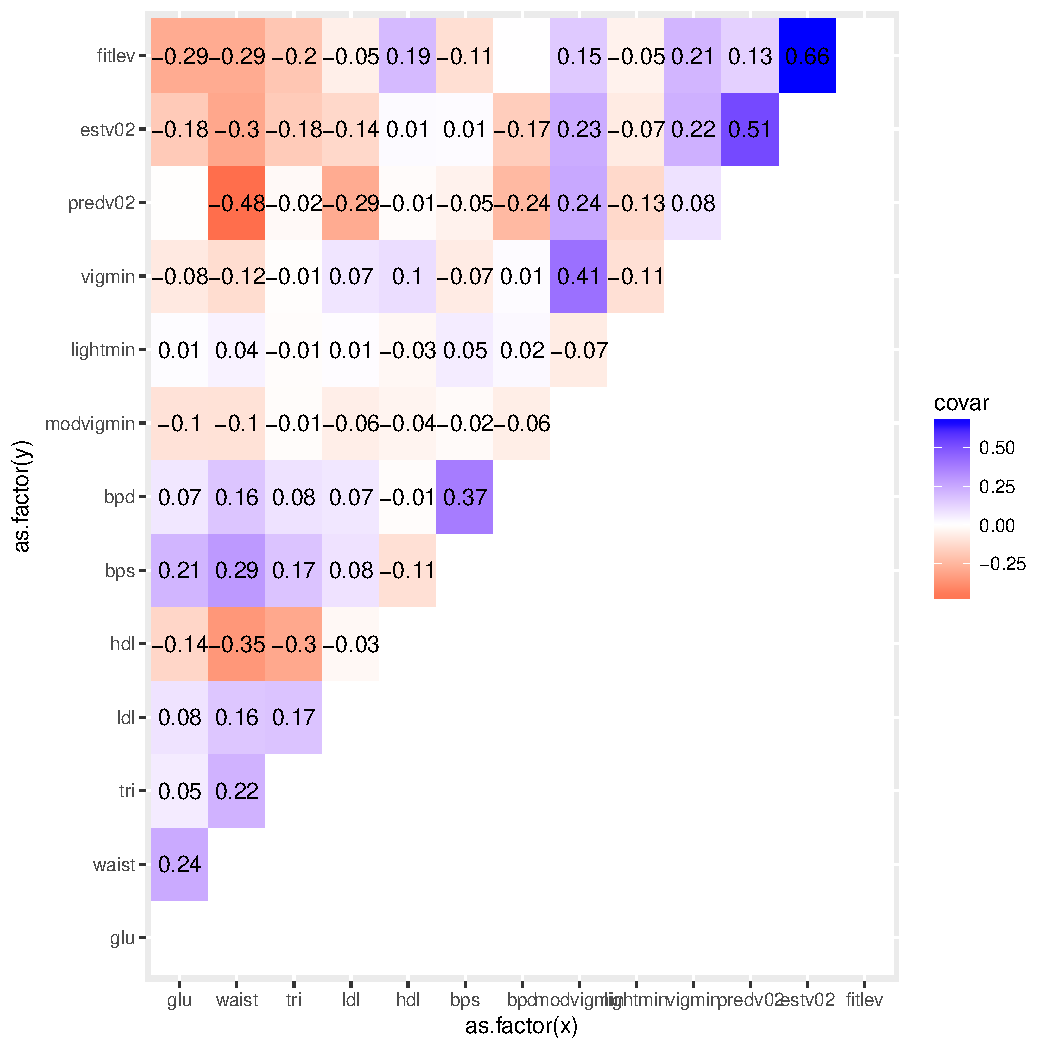
\includegraphics[width=\maxwidth]{figure/c7-1} 

\end{knitrout}


\begin{knitrout}
\definecolor{shadecolor}{rgb}{0.969, 0.969, 0.969}\color{fgcolor}\begin{kframe}
\begin{alltt}
\hlcom{#multivariate regression on mean observed modvig, light}
\hlstd{a} \hlkwb{<-} \hlstd{nhanes} \hlopt \hlkwd{group_by}\hlstd{(id)} \hlopt \hlkwd{summarise}\hlstd{(}\hlkwc{modvig}\hlstd{=}\hlkwd{mean}\hlstd{(modvigmin),}\hlkwc{light}\hlstd{=}\hlkwd{mean}\hlstd{(lightmin))}
\hlstd{y}\hlopt{$}\hlstd{modvig} \hlkwb{<-} \hlstd{a}\hlopt{$}\hlstd{modvig}
\hlstd{y}\hlopt{$}\hlstd{light} \hlkwb{<-} \hlstd{a}\hlopt{$}\hlstd{light}

\hlstd{m3} \hlkwb{<-} \hlkwd{lm}\hlstd{(}\hlkwd{with}\hlstd{(y,}\hlkwd{cbind}\hlstd{(glu,waist,tri,hdl,bps,bpd))}\hlopt{~}\hlstd{y}\hlopt{$}\hlstd{modvig)}
\hlkwd{summary}\hlstd{(m3)}
\end{alltt}
\begin{verbatim}
## Response glu :
## 
## Call:
## lm(formula = glu ~ y$modvig)
## 
## Residuals:
##    Min     1Q Median     3Q    Max 
## -62.50 -14.31  -6.71   2.63 440.78 
## 
## Coefficients:
##              Estimate Std. Error t value Pr(>|t|)    
## (Intercept) 107.87227    0.74640 144.524   <2e-16 ***
## y$modvig     -0.18519    0.02181  -8.491   <2e-16 ***
## ---
## Signif. codes:  0 '***' 0.001 '**' 0.01 '*' 0.05 '.' 0.1 ' ' 1
## 
## Residual standard error: 32.92 on 3574 degrees of freedom
##   (4668 observations deleted due to missingness)
## Multiple R-squared:  0.01977,	Adjusted R-squared:  0.0195 
## F-statistic:  72.1 on 1 and 3574 DF,  p-value: < 2.2e-16
## 
## 
## Response waist :
## 
## Call:
## lm(formula = waist ~ y$modvig)
## 
## Residuals:
##     Min      1Q  Median      3Q     Max 
## -37.507 -10.795  -1.156   9.475  58.162 
## 
## Coefficients:
##              Estimate Std. Error t value Pr(>|t|)    
## (Intercept) 100.19115    0.34288  292.20   <2e-16 ***
## y$modvig     -0.12379    0.01002  -12.36   <2e-16 ***
## ---
## Signif. codes:  0 '***' 0.001 '**' 0.01 '*' 0.05 '.' 0.1 ' ' 1
## 
## Residual standard error: 15.12 on 3574 degrees of freedom
##   (4668 observations deleted due to missingness)
## Multiple R-squared:  0.04096,	Adjusted R-squared:  0.0407 
## F-statistic: 152.7 on 1 and 3574 DF,  p-value: < 2.2e-16
## 
## 
## Response tri :
## 
## Call:
## lm(formula = tri ~ y$modvig)
## 
## Residuals:
##     Min      1Q  Median      3Q     Max 
## -121.18  -65.00  -30.59   27.40 2585.85 
## 
## Coefficients:
##              Estimate Std. Error t value Pr(>|t|)    
## (Intercept) 154.32305    2.85134  54.123  < 2e-16 ***
## y$modvig     -0.40685    0.08331  -4.883 1.09e-06 ***
## ---
## Signif. codes:  0 '***' 0.001 '**' 0.01 '*' 0.05 '.' 0.1 ' ' 1
## 
## Residual standard error: 125.7 on 3574 degrees of freedom
##   (4668 observations deleted due to missingness)
## Multiple R-squared:  0.006628,	Adjusted R-squared:  0.00635 
## F-statistic: 23.85 on 1 and 3574 DF,  p-value: 1.089e-06
## 
## 
## Response hdl :
## 
## Call:
## lm(formula = hdl ~ y$modvig)
## 
## Residuals:
##     Min      1Q  Median      3Q     Max 
## -38.675 -11.922  -2.698   9.320 132.359 
## 
## Coefficients:
##             Estimate Std. Error t value Pr(>|t|)    
## (Intercept)  55.6949     0.3695 150.740   <2e-16 ***
## y$modvig     -0.0233     0.0108  -2.158    0.031 *  
## ---
## Signif. codes:  0 '***' 0.001 '**' 0.01 '*' 0.05 '.' 0.1 ' ' 1
## 
## Residual standard error: 16.29 on 3574 degrees of freedom
##   (4668 observations deleted due to missingness)
## Multiple R-squared:  0.001302,	Adjusted R-squared:  0.001022 
## F-statistic: 4.658 on 1 and 3574 DF,  p-value: 0.03097
## 
## 
## Response bps :
## 
## Call:
## lm(formula = bps ~ y$modvig)
## 
## Residuals:
##     Min      1Q  Median      3Q     Max 
## -44.510 -13.122  -2.921  10.172  93.694 
## 
## Coefficients:
##              Estimate Std. Error t value Pr(>|t|)    
## (Intercept) 126.33975    0.43377  291.26   <2e-16 ***
## y$modvig     -0.13340    0.01267  -10.53   <2e-16 ***
## ---
## Signif. codes:  0 '***' 0.001 '**' 0.01 '*' 0.05 '.' 0.1 ' ' 1
## 
## Residual standard error: 19.13 on 3574 degrees of freedom
##   (4668 observations deleted due to missingness)
## Multiple R-squared:  0.03006,	Adjusted R-squared:  0.02979 
## F-statistic: 110.8 on 1 and 3574 DF,  p-value: < 2.2e-16
## 
## 
## Response bpd :
## 
## Call:
## lm(formula = bpd ~ y$modvig)
## 
## Residuals:
##     Min      1Q  Median      3Q     Max 
## -68.064  -7.423   0.529   8.164  47.533 
## 
## Coefficients:
##              Estimate Std. Error t value Pr(>|t|)    
## (Intercept) 67.729506   0.310267 218.294   <2e-16 ***
## y$modvig     0.013836   0.009066   1.526    0.127    
## ---
## Signif. codes:  0 '***' 0.001 '**' 0.01 '*' 0.05 '.' 0.1 ' ' 1
## 
## Residual standard error: 13.68 on 3574 degrees of freedom
##   (4668 observations deleted due to missingness)
## Multiple R-squared:  0.0006513,	Adjusted R-squared:  0.0003717 
## F-statistic: 2.329 on 1 and 3574 DF,  p-value: 0.1271
\end{verbatim}
\end{kframe}
\end{knitrout}

\begin{knitrout}
\definecolor{shadecolor}{rgb}{0.969, 0.969, 0.969}\color{fgcolor}\begin{kframe}


{\ttfamily\noindent\itshape\color{messagecolor}{\#\# Using\ \ as id variables}}

{\ttfamily\noindent\itshape\color{messagecolor}{\#\# `stat\_bin()` using `bins = 30`. Pick better value with `binwidth`.}}

{\ttfamily\noindent\color{warningcolor}{\#\# Warning: Removed 14799 rows containing non-finite values (stat\_bin).}}\end{kframe}
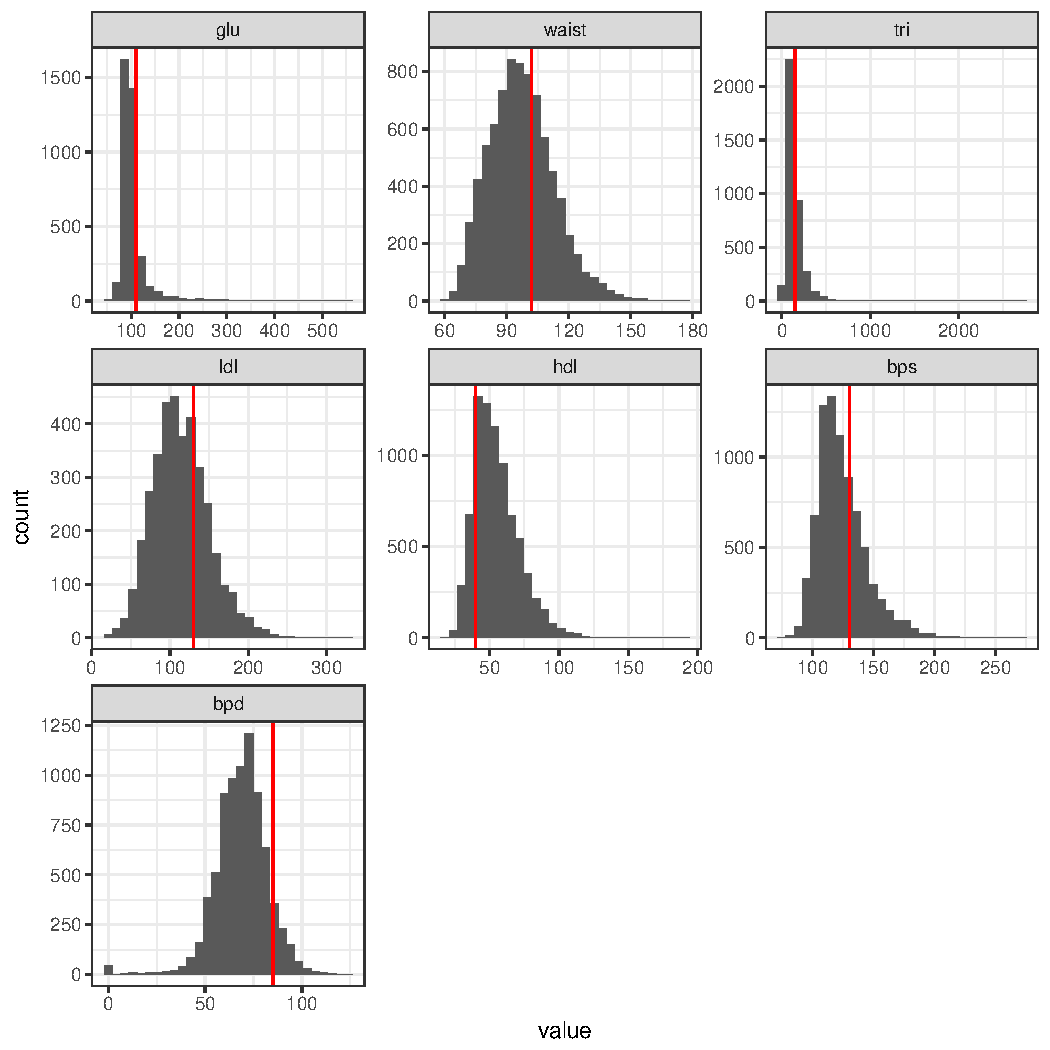
\includegraphics[width=\maxwidth]{figure/c9-1} 

\end{knitrout}

\begin{knitrout}
\definecolor{shadecolor}{rgb}{0.969, 0.969, 0.969}\color{fgcolor}\begin{kframe}


{\ttfamily\noindent\itshape\color{messagecolor}{\#\# `stat\_bin()` using `bins = 30`. Pick better value with `binwidth`.\\\#\# `stat\_bin()` using `bins = 30`. Pick better value with `binwidth`.\\\#\# `stat\_bin()` using `bins = 30`. Pick better value with `binwidth`.}}\end{kframe}
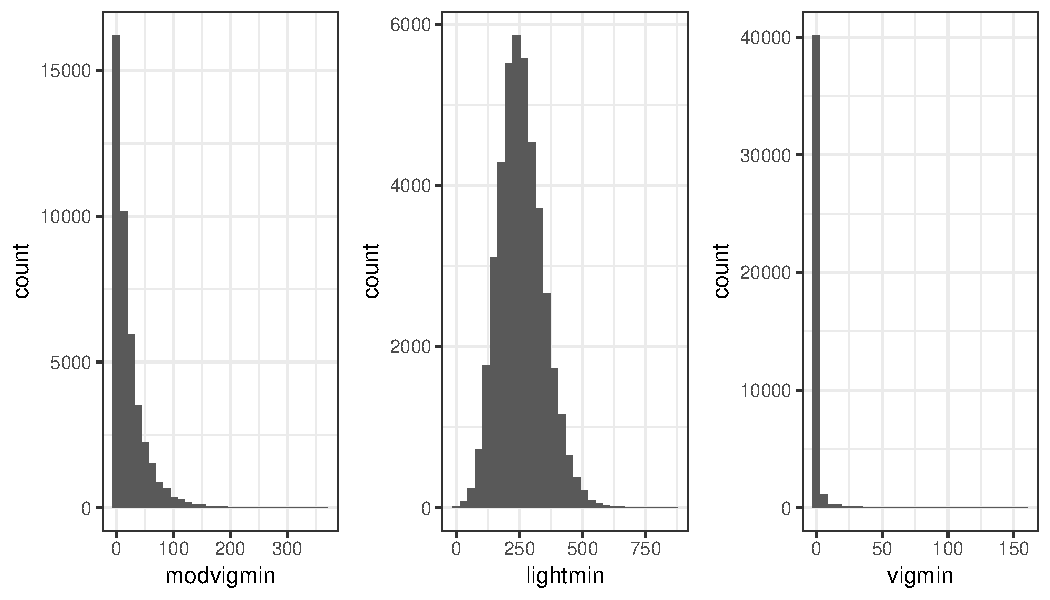
\includegraphics[width=\maxwidth]{figure/c10-1} 

\end{knitrout}

\begin{knitrout}
\definecolor{shadecolor}{rgb}{0.969, 0.969, 0.969}\color{fgcolor}\begin{kframe}
\begin{alltt}
\hlkwd{summary}\hlstd{(}\hlkwd{lm}\hlstd{(wearmin}\hlopt{~}\hlkwd{as.factor}\hlstd{(dow),}\hlkwc{data}\hlstd{=nhanes))}
\end{alltt}
\begin{verbatim}
## 
## Call:
## lm(formula = wearmin ~ as.factor(dow), data = nhanes)
## 
## Residuals:
##     Min      1Q  Median      3Q     Max 
## -261.67 -108.24  -10.55   86.38  621.12 
## 
## Coefficients:
##                 Estimate Std. Error t value Pr(>|t|)    
## (Intercept)      818.882      2.048 399.784  < 2e-16 ***
## as.factor(dow)2   36.599      2.764  13.240  < 2e-16 ***
## as.factor(dow)3   39.281      2.750  14.282  < 2e-16 ***
## as.factor(dow)4   40.428      2.764  14.629  < 2e-16 ***
## as.factor(dow)5   34.328      2.762  12.427  < 2e-16 ***
## as.factor(dow)6   42.792      2.784  15.373  < 2e-16 ***
## as.factor(dow)7   21.738      2.873   7.566 3.92e-14 ***
## ---
## Signif. codes:  0 '***' 0.001 '**' 0.01 '*' 0.05 '.' 0.1 ' ' 1
## 
## Residual standard error: 148.1 on 42433 degrees of freedom
## Multiple R-squared:  0.008106,	Adjusted R-squared:  0.007965 
## F-statistic: 57.79 on 6 and 42433 DF,  p-value: < 2.2e-16
\end{verbatim}
\begin{alltt}
\hlkwd{summary}\hlstd{(}\hlkwd{lm}\hlstd{(wearmin}\hlopt{~}\hlkwd{as.factor}\hlstd{(rep),}\hlkwc{data}\hlstd{=nhanes))}
\end{alltt}
\begin{verbatim}
## 
## Call:
## lm(formula = wearmin ~ as.factor(rep), data = nhanes)
## 
## Residuals:
##     Min      1Q  Median      3Q     Max 
## -258.59 -109.09  -11.53   87.27  615.71 
## 
## Coefficients:
##                 Estimate Std. Error t value Pr(>|t|)    
## (Intercept)      850.727      1.822 466.907  < 2e-16 ***
## as.factor(rep)2    7.868      2.581   3.048  0.00231 ** 
## as.factor(rep)3    5.366      2.599   2.065  0.03893 *  
## as.factor(rep)4    5.782      2.614   2.212  0.02700 *  
## as.factor(rep)5    2.224      2.638   0.843  0.39906    
## as.factor(rep)6   -2.202      2.684  -0.820  0.41198    
## as.factor(rep)7  -26.440      2.807  -9.420  < 2e-16 ***
## ---
## Signif. codes:  0 '***' 0.001 '**' 0.01 '*' 0.05 '.' 0.1 ' ' 1
## 
## Residual standard error: 148.4 on 42433 degrees of freedom
## Multiple R-squared:  0.004513,	Adjusted R-squared:  0.004372 
## F-statistic: 32.06 on 6 and 42433 DF,  p-value: < 2.2e-16
\end{verbatim}
\begin{alltt}
\hlkwd{table}\hlstd{(nhanes}\hlopt{$}\hlstd{rep,nhanes}\hlopt{$}\hlstd{dow)}
\end{alltt}
\begin{verbatim}
##    
##        1    2    3    4    5    6    7
##   1 1507 1482 1180  547  586  543  786
##   2  722 1700 1458 1124  512  567  502
##   3  451  797 1687 1378 1102  480  516
##   4  473  503  789 1638 1368 1062  430
##   5  398  529  486  776 1624 1294  945
##   6  830  472  513  465  764 1545 1080
##   7  847  882  398  445  429  683 1145
\end{verbatim}
\end{kframe}
\end{knitrout}

\begin{knitrout}
\definecolor{shadecolor}{rgb}{0.969, 0.969, 0.969}\color{fgcolor}\begin{kframe}
\begin{alltt}
\hlkwd{dim}\hlstd{(nhanes)}
\end{alltt}
\begin{verbatim}
## [1] 42440    39
\end{verbatim}
\begin{alltt}
\hlkwd{length}\hlstd{(}\hlkwd{unique}\hlstd{(nhanes}\hlopt{$}\hlstd{id))}
\end{alltt}
\begin{verbatim}
## [1] 8244
\end{verbatim}
\begin{alltt}
\hlkwd{table}\hlstd{(nrep)} \hlcom{#gives distribution of number of replicates}
\end{alltt}
\begin{verbatim}
## nrep
##    1    2    3    4    5    6    7 
##  510  555  656  834 1249 1809 2631
\end{verbatim}
\begin{alltt}
\hlstd{meas7} \hlkwb{<-} \hlkwd{subset}\hlstd{(nhanes, id} \hlopt \hlkwd{unique}\hlstd{(id)[nrep}\hlopt{==}\hlnum{7}\hlstd{])} \hlcom{#individuals with all 7 days}
\hlkwd{length}\hlstd{(}\hlkwd{unique}\hlstd{(meas7}\hlopt{$}\hlstd{id[}\hlkwd{complete.cases}\hlstd{(meas7[,}\hlkwd{c}\hlstd{(}\hlstr{"smplwt"}\hlstd{,}\hlstr{"sex"}\hlstd{,}\hlstr{"age"}\hlstd{,}\hlstr{"race"}\hlstd{,}\hlstr{"rep"}\hlstd{,}\hlstr{"dow"}\hlstd{,}\hlstr{"wearmin"}\hlstd{,}\hlstr{"modvigmin"}\hlstd{,}\hlstr{"modvigminb"}\hlstd{,}\hlstr{"modvigbouts"}\hlstd{,}\hlstr{"glu"}\hlstd{,}\hlstr{"waist"}\hlstd{,}\hlstr{"tri"}\hlstd{,}\hlstr{"ldl"}\hlstd{,}\hlstr{"hdl"}\hlstd{,}\hlstr{"bps"}\hlstd{,}\hlstr{"bpd"}\hlstd{)])]))} \hlcom{#with bpmed 405}
\end{alltt}
\begin{verbatim}
## [1] 1103
\end{verbatim}
\begin{alltt}
\hlcom{#no big changes by taking one of the 7 metsynd variables out}

\hlstd{id7complete} \hlkwb{<-} \hlkwd{unique}\hlstd{(meas7}\hlopt{$}\hlstd{id[}\hlkwd{complete.cases}\hlstd{(meas7[,}\hlkwd{c}\hlstd{(}\hlstr{"smplwt"}\hlstd{,}\hlstr{"sex"}\hlstd{,}\hlstr{"age"}\hlstd{,}\hlstr{"race"}\hlstd{,}\hlstr{"rep"}\hlstd{,}\hlstr{"dow"}\hlstd{,}\hlstr{"wearmin"}\hlstd{,}\hlstr{"modvigmin"}\hlstd{,}\hlstr{"modvigminb"}\hlstd{,}\hlstr{"modvigbouts"}\hlstd{,}\hlstr{"glu"}\hlstd{,}\hlstr{"waist"}\hlstd{,}\hlstr{"tri"}\hlstd{,}\hlstr{"ldl"}\hlstd{,}\hlstr{"hdl"}\hlstd{,}\hlstr{"bps"}\hlstd{,}\hlstr{"bpd"}\hlstd{)])])}

\hlstd{meas67} \hlkwb{<-} \hlkwd{subset}\hlstd{(nhanes, id} \hlopt \hlkwd{unique}\hlstd{(id)[nrep}\hlopt{>=}\hlnum{6}\hlstd{]} \hlopt{&} \hlstd{rep} \hlopt{<=} \hlnum{6}\hlstd{)} \hlcom{#individuals with 6 days}
\hlkwd{length}\hlstd{(}\hlkwd{unique}\hlstd{(meas67}\hlopt{$}\hlstd{id[}\hlkwd{complete.cases}\hlstd{(meas67[,}\hlkwd{c}\hlstd{(}\hlstr{"smplwt"}\hlstd{,}\hlstr{"sex"}\hlstd{,}\hlstr{"age"}\hlstd{,}\hlstr{"race"}\hlstd{,}\hlstr{"rep"}\hlstd{,}\hlstr{"dow"}\hlstd{,}\hlstr{"wearmin"}\hlstd{,}\hlstr{"modvigmin"}\hlstd{,}\hlstr{"modvigminb"}\hlstd{,}\hlstr{"modvigbouts"}\hlstd{,}\hlstr{"glu"}\hlstd{,}\hlstr{"waist"}\hlstd{,}\hlstr{"tri"}\hlstd{,}\hlstr{"ldl"}\hlstd{,}\hlstr{"hdl"}\hlstd{,}\hlstr{"bps"}\hlstd{,}\hlstr{"bpd"}\hlstd{)])]))} \hlcom{#with bpmed 638}
\end{alltt}
\begin{verbatim}
## [1] 1878
\end{verbatim}
\begin{alltt}
\hlstd{meas57} \hlkwb{<-} \hlkwd{subset}\hlstd{(nhanes, id} \hlopt \hlkwd{unique}\hlstd{(id)[nrep}\hlopt{>=}\hlnum{5}\hlstd{]} \hlopt{&} \hlstd{rep} \hlopt{<=} \hlnum{5}\hlstd{)} \hlcom{#individuals with 6 days}
\hlkwd{length}\hlstd{(}\hlkwd{unique}\hlstd{(meas57}\hlopt{$}\hlstd{id[}\hlkwd{complete.cases}\hlstd{(meas57[,}\hlkwd{c}\hlstd{(}\hlstr{"smplwt"}\hlstd{,}\hlstr{"sex"}\hlstd{,}\hlstr{"age"}\hlstd{,}\hlstr{"race"}\hlstd{,}\hlstr{"rep"}\hlstd{,}\hlstr{"dow"}\hlstd{,}\hlstr{"wearmin"}\hlstd{,}\hlstr{"modvigmin"}\hlstd{,}\hlstr{"modvigminb"}\hlstd{,}\hlstr{"modvigbouts"}\hlstd{,}\hlstr{"glu"}\hlstd{,}\hlstr{"waist"}\hlstd{,}\hlstr{"tri"}\hlstd{,}\hlstr{"ldl"}\hlstd{,}\hlstr{"hdl"}\hlstd{,}\hlstr{"bps"}\hlstd{,}\hlstr{"bpd"}\hlstd{)])]))} \hlcom{#with bpmed 803, 348 estv02}
\end{alltt}
\begin{verbatim}
## [1] 2424
\end{verbatim}
\begin{alltt}
\hlstd{id57complete} \hlkwb{<-} \hlkwd{unique}\hlstd{(meas57}\hlopt{$}\hlstd{id[}\hlkwd{complete.cases}\hlstd{(meas57[,}\hlkwd{c}\hlstd{(}\hlstr{"smplwt"}\hlstd{,}\hlstr{"sex"}\hlstd{,}\hlstr{"age"}\hlstd{,}\hlstr{"race"}\hlstd{,}\hlstr{"rep"}\hlstd{,}\hlstr{"dow"}\hlstd{,}\hlstr{"wearmin"}\hlstd{,}\hlstr{"modvigmin"}\hlstd{,}\hlstr{"modvigminb"}\hlstd{,}\hlstr{"modvigbouts"}\hlstd{,}\hlstr{"glu"}\hlstd{,}\hlstr{"waist"}\hlstd{,}\hlstr{"tri"}\hlstd{,}\hlstr{"ldl"}\hlstd{,}\hlstr{"hdl"}\hlstd{,}\hlstr{"bps"}\hlstd{,}\hlstr{"bpd"}\hlstd{)])])}

\hlkwd{table}\hlstd{((meas57} \hlopt \hlkwd{group_by}\hlstd{(id)} \hlopt \hlkwd{summarise}\hlstd{(}\hlkwc{n}\hlstd{=}\hlkwd{length}\hlstd{(id)))}\hlopt{$}\hlstd{n)}
\end{alltt}
\begin{verbatim}
## 
##    3    4    5 
##  333 1510 3846
\end{verbatim}
\begin{alltt}
\hlkwd{table}\hlstd{((meas67} \hlopt \hlkwd{group_by}\hlstd{(id)} \hlopt \hlkwd{summarise}\hlstd{(}\hlkwc{n}\hlstd{=}\hlkwd{length}\hlstd{(id)))}\hlopt{$}\hlstd{n)}
\end{alltt}
\begin{verbatim}
## 
##    5    6 
## 1088 3352
\end{verbatim}
\end{kframe}
\end{knitrout}


\begin{knitrout}
\definecolor{shadecolor}{rgb}{0.969, 0.969, 0.969}\color{fgcolor}\begin{kframe}
\begin{alltt}
\hlstd{q1} \hlkwb{<-} \hlkwd{lm}\hlstd{(modvigmin}\hlopt{~}\hlkwd{as.factor}\hlstd{(rep),}\hlkwc{data}\hlstd{=nhanes)}
\hlstd{nhanes}\hlopt{$}\hlstd{rep2} \hlkwb{<-} \hlstd{nhanes}\hlopt{$}\hlstd{rep}
\hlstd{nhanes}\hlopt{$}\hlstd{rep2[nhanes}\hlopt{$}\hlstd{rep} \hlopt \hlkwd{c}\hlstd{(}\hlnum{1}\hlopt{:}\hlnum{5}\hlstd{)]} \hlkwb{<-} \hlnum{1}
\hlstd{q2} \hlkwb{<-} \hlkwd{lm}\hlstd{(modvigmin}\hlopt{~}\hlkwd{as.factor}\hlstd{(rep2),}\hlkwc{data}\hlstd{=nhanes)}
\hlkwd{anova}\hlstd{(q1,q2)}
\end{alltt}
\begin{verbatim}
## Analysis of Variance Table
## 
## Model 1: modvigmin ~ as.factor(rep)
## Model 2: modvigmin ~ as.factor(rep2)
##   Res.Df      RSS Df Sum of Sq      F Pr(>F)
## 1  42433 35902020                           
## 2  42437 35904922 -4   -2901.8 0.8574 0.4887
\end{verbatim}
\begin{alltt}
\hlstd{q3} \hlkwb{<-} \hlkwd{lm}\hlstd{(modvigmin}\hlopt{~}\hlkwd{as.factor}\hlstd{(dow),}\hlkwc{data}\hlstd{=nhanes)}
\hlstd{q4} \hlkwb{<-} \hlkwd{lm}\hlstd{(modvigmin}\hlopt{~}\hlkwd{as.factor}\hlstd{(weekend),}\hlkwc{data}\hlstd{=nhanes)}
\hlstd{nhanes}\hlopt{$}\hlstd{dow2} \hlkwb{<-} \hlstd{nhanes}\hlopt{$}\hlstd{dow}
\hlstd{nhanes}\hlopt{$}\hlstd{dow2[nhanes}\hlopt{$}\hlstd{dow} \hlopt \hlkwd{c}\hlstd{(}\hlnum{2}\hlopt{:}\hlnum{6}\hlstd{)]} \hlkwb{<-} \hlnum{2}
\hlstd{q5} \hlkwb{<-} \hlkwd{lm}\hlstd{(modvigmin}\hlopt{~}\hlkwd{as.factor}\hlstd{(dow2),}\hlkwc{data}\hlstd{=nhanes)}

\hlkwd{anova}\hlstd{(q3,q4)}
\end{alltt}
\begin{verbatim}
## Analysis of Variance Table
## 
## Model 1: modvigmin ~ as.factor(dow)
## Model 2: modvigmin ~ as.factor(weekend)
##   Res.Df      RSS Df Sum of Sq      F    Pr(>F)    
## 1  42433 35755786                                  
## 2  42438 35773439 -5    -17653 4.1899 0.0008297 ***
## ---
## Signif. codes:  0 '***' 0.001 '**' 0.01 '*' 0.05 '.' 0.1 ' ' 1
\end{verbatim}
\begin{alltt}
\hlkwd{anova}\hlstd{(q3,q5)}
\end{alltt}
\begin{verbatim}
## Analysis of Variance Table
## 
## Model 1: modvigmin ~ as.factor(dow)
## Model 2: modvigmin ~ as.factor(dow2)
##   Res.Df      RSS Df Sum of Sq      F Pr(>F)
## 1  42433 35755786                           
## 2  42437 35762149 -4     -6363 1.8878 0.1095
\end{verbatim}
\begin{alltt}
\hlstd{q1} \hlkwb{<-} \hlkwd{lm}\hlstd{(modvigmin}\hlopt{~}\hlkwd{as.factor}\hlstd{(rep),}\hlkwc{data}\hlstd{=meas7)}
\hlstd{meas7}\hlopt{$}\hlstd{rep2} \hlkwb{<-} \hlstd{meas7}\hlopt{$}\hlstd{rep}
\hlstd{meas7}\hlopt{$}\hlstd{rep2[meas7}\hlopt{$}\hlstd{rep} \hlopt \hlkwd{c}\hlstd{(}\hlnum{1}\hlopt{:}\hlnum{5}\hlstd{)]} \hlkwb{<-} \hlnum{1}
\hlstd{q2} \hlkwb{<-} \hlkwd{lm}\hlstd{(modvigmin}\hlopt{~}\hlkwd{as.factor}\hlstd{(rep2),}\hlkwc{data}\hlstd{=meas7)}
\hlkwd{anova}\hlstd{(q1,q2)}
\end{alltt}
\begin{verbatim}
## Analysis of Variance Table
## 
## Model 1: modvigmin ~ as.factor(rep)
## Model 2: modvigmin ~ as.factor(rep2)
##   Res.Df      RSS Df Sum of Sq      F Pr(>F)
## 1  18410 14037352                           
## 2  18414 14038137 -4   -785.07 0.2574 0.9053
\end{verbatim}
\begin{alltt}
\hlstd{q3} \hlkwb{<-} \hlkwd{lm}\hlstd{(modvigmin}\hlopt{~}\hlkwd{as.factor}\hlstd{(dow),}\hlkwc{data}\hlstd{=meas7)}
\hlstd{q4} \hlkwb{<-} \hlkwd{lm}\hlstd{(modvigmin}\hlopt{~}\hlkwd{as.factor}\hlstd{(weekend),}\hlkwc{data}\hlstd{=meas7)}
\hlstd{meas7}\hlopt{$}\hlstd{dow2} \hlkwb{<-} \hlstd{meas7}\hlopt{$}\hlstd{dow}
\hlstd{meas7}\hlopt{$}\hlstd{dow2[meas7}\hlopt{$}\hlstd{dow} \hlopt \hlkwd{c}\hlstd{(}\hlnum{2}\hlopt{:}\hlnum{6}\hlstd{)]} \hlkwb{<-} \hlnum{2}
\hlstd{q5} \hlkwb{<-} \hlkwd{lm}\hlstd{(modvigmin}\hlopt{~}\hlkwd{as.factor}\hlstd{(dow2),}\hlkwc{data}\hlstd{=meas7)}

\hlkwd{anova}\hlstd{(q3,q4)}
\end{alltt}
\begin{verbatim}
## Analysis of Variance Table
## 
## Model 1: modvigmin ~ as.factor(dow)
## Model 2: modvigmin ~ as.factor(weekend)
##   Res.Df      RSS Df Sum of Sq     F Pr(>F)
## 1  18410 13976558                          
## 2  18415 13983155 -5   -6597.3 1.738 0.1221
\end{verbatim}
\begin{alltt}
\hlkwd{anova}\hlstd{(q3,q5)}
\end{alltt}
\begin{verbatim}
## Analysis of Variance Table
## 
## Model 1: modvigmin ~ as.factor(dow)
## Model 2: modvigmin ~ as.factor(dow2)
##   Res.Df      RSS Df Sum of Sq      F Pr(>F)
## 1  18410 13976558                           
## 2  18414 13977073 -4   -515.62 0.1698 0.9539
\end{verbatim}
\end{kframe}
\end{knitrout}


\begin{knitrout}
\definecolor{shadecolor}{rgb}{0.969, 0.969, 0.969}\color{fgcolor}\begin{kframe}
\begin{alltt}
\hlstd{m1a} \hlkwb{<-} \hlkwd{gls}\hlstd{(modvigmin}\hlopt{~}\hlkwd{as.factor}\hlstd{(dow)}\hlopt{+}\hlkwd{as.factor}\hlstd{(rep),}\hlkwc{data}\hlstd{=meas7,}\hlkwc{correlation}\hlstd{=}\hlkwd{corCompSymm}\hlstd{(}\hlkwc{form}\hlstd{=}\hlopt{~}\hlnum{1}\hlopt{|}\hlstd{id),}\hlkwc{method}\hlstd{=}\hlstr{"ML"}\hlstd{)}
\hlstd{m2a} \hlkwb{<-} \hlkwd{gls}\hlstd{(modvigmin}\hlopt{~}\hlkwd{as.factor}\hlstd{(dow)}\hlopt{+}\hlkwd{as.factor}\hlstd{(rep),}\hlkwc{data}\hlstd{=meas7,}\hlkwc{correlation}\hlstd{=}\hlkwd{corAR1}\hlstd{(}\hlkwc{form}\hlstd{=}\hlopt{~}\hlnum{1}\hlopt{|}\hlstd{id),}\hlkwc{method}\hlstd{=}\hlstr{"ML"}\hlstd{)}
\hlstd{m3a} \hlkwb{<-} \hlkwd{gls}\hlstd{(modvigmin}\hlopt{~}\hlkwd{as.factor}\hlstd{(dow)}\hlopt{+}\hlkwd{as.factor}\hlstd{(rep),}\hlkwc{data}\hlstd{=meas7,}\hlkwc{correlation}\hlstd{=}\hlkwd{corARMA}\hlstd{(}\hlkwc{form}\hlstd{=}\hlopt{~}\hlnum{1}\hlopt{|}\hlstd{id,}\hlkwc{p}\hlstd{=}\hlnum{1}\hlstd{,}\hlkwc{q}\hlstd{=}\hlnum{1}\hlstd{),}\hlkwc{method}\hlstd{=}\hlstr{"ML"}\hlstd{)}
\hlstd{m4a} \hlkwb{<-} \hlkwd{gls}\hlstd{(modvigmin}\hlopt{~}\hlkwd{as.factor}\hlstd{(dow)}\hlopt{+}\hlkwd{as.factor}\hlstd{(rep),}\hlkwc{data}\hlstd{=meas7,}\hlkwc{correlation}\hlstd{=}\hlkwd{corARMA}\hlstd{(}\hlkwc{form}\hlstd{=}\hlopt{~}\hlnum{1}\hlopt{|}\hlstd{id,}\hlkwc{p}\hlstd{=}\hlnum{2}\hlstd{,}\hlkwc{q}\hlstd{=}\hlnum{0}\hlstd{),}\hlkwc{method}\hlstd{=}\hlstr{"ML"}\hlstd{)}
\hlstd{m6a} \hlkwb{<-} \hlkwd{gls}\hlstd{(modvigmin}\hlopt{~}\hlkwd{as.factor}\hlstd{(dow)}\hlopt{+}\hlkwd{as.factor}\hlstd{(rep),}\hlkwc{data}\hlstd{=meas7,}\hlkwc{correlation}\hlstd{=}\hlkwd{corARMA}\hlstd{(}\hlkwc{form}\hlstd{=}\hlopt{~}\hlnum{1}\hlopt{|}\hlstd{id,}\hlkwc{p}\hlstd{=}\hlnum{2}\hlstd{,}\hlkwc{q}\hlstd{=}\hlnum{1}\hlstd{),}\hlkwc{method}\hlstd{=}\hlstr{"ML"}\hlstd{)}
\hlstd{m7a} \hlkwb{<-} \hlkwd{gls}\hlstd{(modvigmin}\hlopt{~}\hlkwd{as.factor}\hlstd{(dow)}\hlopt{+}\hlkwd{as.factor}\hlstd{(rep),}\hlkwc{data}\hlstd{=meas7,}\hlkwc{correlation}\hlstd{=}\hlkwd{corSymm}\hlstd{(}\hlkwc{form}\hlstd{=}\hlopt{~}\hlnum{1}\hlopt{|}\hlstd{id),}\hlkwc{method}\hlstd{=}\hlstr{"ML"}\hlstd{)}
\hlstd{m8a} \hlkwb{<-} \hlkwd{gls}\hlstd{(modvigmin}\hlopt{~}\hlkwd{as.factor}\hlstd{(dow)}\hlopt{+}\hlkwd{as.factor}\hlstd{(rep),}\hlkwc{data}\hlstd{=meas7,}\hlkwc{correlation}\hlstd{=}\hlkwd{corSymm}\hlstd{(}\hlkwc{form}\hlstd{=}\hlopt{~}\hlnum{1}\hlopt{|}\hlstd{id),}\hlkwc{weight} \hlstd{=} \hlkwd{varIdent}\hlstd{(}\hlkwc{form} \hlstd{=} \hlopt{~} \hlnum{1}\hlopt{|}\hlstd{rep),}\hlkwc{method}\hlstd{=}\hlstr{"ML"}\hlstd{)}

\hlkwd{extractAIC}\hlstd{(m1a)}
\end{alltt}
\begin{verbatim}
## [1]     15.0 164398.1
\end{verbatim}
\begin{alltt}
\hlkwd{extractAIC}\hlstd{(m2a)}
\end{alltt}
\begin{verbatim}
## [1]     15.0 166262.7
\end{verbatim}
\begin{alltt}
\hlkwd{extractAIC}\hlstd{(m3a)}
\end{alltt}
\begin{verbatim}
## [1]     16.0 164252.2
\end{verbatim}
\begin{alltt}
\hlkwd{extractAIC}\hlstd{(m4a)}
\end{alltt}
\begin{verbatim}
## [1]     16.0 164938.2
\end{verbatim}
\begin{alltt}
\hlkwd{extractAIC}\hlstd{(m6a)}
\end{alltt}
\begin{verbatim}
## [1]     17.0 164181.5
\end{verbatim}
\begin{alltt}
\hlkwd{extractAIC}\hlstd{(m7a)}
\end{alltt}
\begin{verbatim}
## [1]     35.0 164043.4
\end{verbatim}
\begin{alltt}
\hlkwd{extractAIC}\hlstd{(m8a)}
\end{alltt}
\begin{verbatim}
## [1]     41.0 164029.9
\end{verbatim}
\begin{alltt}
\hlkwd{anova}\hlstd{(m3a,m2a)}
\end{alltt}
\begin{verbatim}
##     Model df      AIC      BIC    logLik   Test  L.Ratio p-value
## m3a     1 16 164252.2 164377.3 -82110.08                        
## m2a     2 15 166262.8 166380.1 -83116.37 1 vs 2 2012.582  <.0001
\end{verbatim}
\begin{alltt}
\hlkwd{anova}\hlstd{(m6a,m3a)}
\end{alltt}
\begin{verbatim}
##     Model df      AIC      BIC    logLik   Test  L.Ratio p-value
## m6a     1 17 164181.5 164314.4 -82073.73                        
## m3a     2 16 164252.2 164377.3 -82110.08 1 vs 2 72.71033  <.0001
\end{verbatim}
\begin{alltt}
\hlkwd{anova}\hlstd{(m7a,m6a)}
\end{alltt}
\begin{verbatim}
##     Model df      AIC      BIC    logLik   Test  L.Ratio p-value
## m7a     1 35 164043.4 164317.1 -81986.68                        
## m6a     2 17 164181.5 164314.4 -82073.73 1 vs 2 174.0954  <.0001
\end{verbatim}
\begin{alltt}
\hlkwd{anova}\hlstd{(m8a,m7a)}
\end{alltt}
\begin{verbatim}
##     Model df      AIC      BIC    logLik   Test  L.Ratio p-value
## m8a     1 41 164029.9 164350.5 -81973.94                        
## m7a     2 35 164043.4 164317.1 -81986.68 1 vs 2 25.47542   3e-04
\end{verbatim}
\end{kframe}
\end{knitrout}

\begin{knitrout}
\definecolor{shadecolor}{rgb}{0.969, 0.969, 0.969}\color{fgcolor}\begin{kframe}
\begin{alltt}
\hlstd{meas57sub} \hlkwb{<-} \hlkwd{subset}\hlstd{(meas57,rep} \hlopt{<=}\hlnum{5}\hlstd{)}

\hlstd{m1b} \hlkwb{<-} \hlkwd{gls}\hlstd{(modvigmin}\hlopt{~}\hlkwd{as.factor}\hlstd{(dow)}\hlopt{+}\hlkwd{as.factor}\hlstd{(rep),}\hlkwc{data}\hlstd{=meas57sub,}\hlkwc{correlation}\hlstd{=}\hlkwd{corCompSymm}\hlstd{(}\hlkwc{form}\hlstd{=}\hlopt{~}\hlnum{1}\hlopt{|}\hlstd{id),}\hlkwc{method}\hlstd{=}\hlstr{"ML"}\hlstd{)}
\hlstd{m2b} \hlkwb{<-} \hlkwd{gls}\hlstd{(modvigmin}\hlopt{~}\hlkwd{as.factor}\hlstd{(dow)}\hlopt{+}\hlkwd{as.factor}\hlstd{(rep),}\hlkwc{data}\hlstd{=meas57sub,}\hlkwc{correlation}\hlstd{=}\hlkwd{corAR1}\hlstd{(}\hlkwc{form}\hlstd{=}\hlopt{~}\hlnum{1}\hlopt{|}\hlstd{id),}\hlkwc{method}\hlstd{=}\hlstr{"ML"}\hlstd{)}
\hlstd{m3b} \hlkwb{<-} \hlkwd{gls}\hlstd{(modvigmin}\hlopt{~}\hlkwd{as.factor}\hlstd{(dow)}\hlopt{+}\hlkwd{as.factor}\hlstd{(rep),}\hlkwc{data}\hlstd{=meas57sub,}\hlkwc{correlation}\hlstd{=}\hlkwd{corARMA}\hlstd{(}\hlkwc{form}\hlstd{=}\hlopt{~}\hlnum{1}\hlopt{|}\hlstd{id,}\hlkwc{p}\hlstd{=}\hlnum{1}\hlstd{,}\hlkwc{q}\hlstd{=}\hlnum{1}\hlstd{),}\hlkwc{method}\hlstd{=}\hlstr{"ML"}\hlstd{)}
\hlstd{m4b} \hlkwb{<-} \hlkwd{gls}\hlstd{(modvigmin}\hlopt{~}\hlkwd{as.factor}\hlstd{(dow)}\hlopt{+}\hlkwd{as.factor}\hlstd{(rep),}\hlkwc{data}\hlstd{=meas57sub,}\hlkwc{correlation}\hlstd{=}\hlkwd{corARMA}\hlstd{(}\hlkwc{form}\hlstd{=}\hlopt{~}\hlnum{1}\hlopt{|}\hlstd{id,}\hlkwc{p}\hlstd{=}\hlnum{2}\hlstd{,}\hlkwc{q}\hlstd{=}\hlnum{0}\hlstd{),}\hlkwc{method}\hlstd{=}\hlstr{"ML"}\hlstd{)}
\hlstd{m6b} \hlkwb{<-} \hlkwd{gls}\hlstd{(modvigmin}\hlopt{~}\hlkwd{as.factor}\hlstd{(dow)}\hlopt{+}\hlkwd{as.factor}\hlstd{(rep),}\hlkwc{data}\hlstd{=meas57sub,}\hlkwc{correlation}\hlstd{=}\hlkwd{corARMA}\hlstd{(}\hlkwc{form}\hlstd{=}\hlopt{~}\hlnum{1}\hlopt{|}\hlstd{id,}\hlkwc{p}\hlstd{=}\hlnum{2}\hlstd{,}\hlkwc{q}\hlstd{=}\hlnum{1}\hlstd{),}\hlkwc{method}\hlstd{=}\hlstr{"ML"}\hlstd{)}
\hlstd{m7b} \hlkwb{<-} \hlkwd{gls}\hlstd{(modvigmin}\hlopt{~}\hlkwd{as.factor}\hlstd{(dow)}\hlopt{+}\hlkwd{as.factor}\hlstd{(rep),}\hlkwc{data}\hlstd{=meas57sub,}\hlkwc{correlation}\hlstd{=}\hlkwd{corSymm}\hlstd{(}\hlkwc{form}\hlstd{=}\hlopt{~}\hlnum{1}\hlopt{|}\hlstd{id),}\hlkwc{method}\hlstd{=}\hlstr{"ML"}\hlstd{)}
\hlstd{m8b} \hlkwb{<-} \hlkwd{gls}\hlstd{(modvigmin}\hlopt{~}\hlkwd{as.factor}\hlstd{(dow)}\hlopt{+}\hlkwd{as.factor}\hlstd{(rep),}\hlkwc{data}\hlstd{=meas57,}\hlkwc{correlation}\hlstd{=}\hlkwd{corSymm}\hlstd{(}\hlkwc{form}\hlstd{=}\hlopt{~}\hlnum{1}\hlopt{|}\hlstd{id),}\hlkwc{weight} \hlstd{=} \hlkwd{varIdent}\hlstd{(}\hlkwc{form} \hlstd{=} \hlopt{~} \hlnum{1}\hlopt{|}\hlstd{rep),}\hlkwc{method}\hlstd{=}\hlstr{"ML"}\hlstd{)}

\hlkwd{extractAIC}\hlstd{(m1b)}
\end{alltt}
\begin{verbatim}
## [1]     13 238400
\end{verbatim}
\begin{alltt}
\hlkwd{extractAIC}\hlstd{(m2b)}
\end{alltt}
\begin{verbatim}
## [1]     13.0 240187.2
\end{verbatim}
\begin{alltt}
\hlkwd{extractAIC}\hlstd{(m3b)}
\end{alltt}
\begin{verbatim}
## [1]     14.0 238171.1
\end{verbatim}
\begin{alltt}
\hlkwd{extractAIC}\hlstd{(m4b)}
\end{alltt}
\begin{verbatim}
## [1]     14.0 238567.7
\end{verbatim}
\begin{alltt}
\hlkwd{extractAIC}\hlstd{(m6b)}
\end{alltt}
\begin{verbatim}
## [1]     15 238171
\end{verbatim}
\begin{alltt}
\hlkwd{extractAIC}\hlstd{(m7b)}
\end{alltt}
\begin{verbatim}
## [1]     22.0 238067.3
\end{verbatim}
\begin{alltt}
\hlkwd{extractAIC}\hlstd{(m8b)}
\end{alltt}
\begin{verbatim}
## [1]     26.0 238041.9
\end{verbatim}
\begin{alltt}
\hlkwd{anova}\hlstd{(m3b,m2b)}
\end{alltt}
\begin{verbatim}
##     Model df      AIC      BIC    logLik   Test  L.Ratio p-value
## m3b     1 14 238171.1 238285.6 -119071.6                        
## m2b     2 13 240187.2 240293.5 -120080.6 1 vs 2 2018.088  <.0001
\end{verbatim}
\begin{alltt}
\hlkwd{anova}\hlstd{(m6b,m3b)}
\end{alltt}
\begin{verbatim}
##     Model df      AIC      BIC    logLik   Test  L.Ratio p-value
## m6b     1 15 238171.0 238293.7 -119070.5                        
## m3b     2 14 238171.1 238285.6 -119071.6 1 vs 2 2.070635  0.1502
\end{verbatim}
\begin{alltt}
\hlkwd{anova}\hlstd{(m7b,m3b)}
\end{alltt}
\begin{verbatim}
##     Model df      AIC      BIC    logLik   Test  L.Ratio p-value
## m7b     1 22 238067.3 238247.2 -119011.6                        
## m3b     2 14 238171.1 238285.6 -119071.6 1 vs 2 119.8111  <.0001
\end{verbatim}
\begin{alltt}
\hlkwd{anova}\hlstd{(m8b,m7b)}
\end{alltt}
\begin{verbatim}
##     Model df      AIC      BIC    logLik   Test  L.Ratio p-value
## m8b     1 26 238041.9 238254.4 -118994.9                        
## m7b     2 22 238067.3 238247.2 -119011.6 1 vs 2 33.45403  <.0001
\end{verbatim}
\end{kframe}
\end{knitrout}

\begin{knitrout}
\definecolor{shadecolor}{rgb}{0.969, 0.969, 0.969}\color{fgcolor}\begin{kframe}
\begin{alltt}
\hlstd{meas67sub} \hlkwb{<-} \hlkwd{subset}\hlstd{(meas67,rep} \hlopt{<=}\hlnum{6}\hlstd{)}

\hlstd{m1c} \hlkwb{<-} \hlkwd{gls}\hlstd{(modvigmin}\hlopt{~}\hlkwd{as.factor}\hlstd{(dow)}\hlopt{+}\hlkwd{as.factor}\hlstd{(rep),}\hlkwc{data}\hlstd{=meas67sub,}\hlkwc{correlation}\hlstd{=}\hlkwd{corCompSymm}\hlstd{(}\hlkwc{form}\hlstd{=}\hlopt{~}\hlnum{1}\hlopt{|}\hlstd{id),}\hlkwc{method}\hlstd{=}\hlstr{"ML"}\hlstd{)}
\hlstd{m2c} \hlkwb{<-} \hlkwd{gls}\hlstd{(modvigmin}\hlopt{~}\hlkwd{as.factor}\hlstd{(dow)}\hlopt{+}\hlkwd{as.factor}\hlstd{(rep),}\hlkwc{data}\hlstd{=meas67sub,}\hlkwc{correlation}\hlstd{=}\hlkwd{corAR1}\hlstd{(}\hlkwc{form}\hlstd{=}\hlopt{~}\hlnum{1}\hlopt{|}\hlstd{id),}\hlkwc{method}\hlstd{=}\hlstr{"ML"}\hlstd{)}
\hlstd{m3c} \hlkwb{<-} \hlkwd{gls}\hlstd{(modvigmin}\hlopt{~}\hlkwd{as.factor}\hlstd{(dow)}\hlopt{+}\hlkwd{as.factor}\hlstd{(rep),}\hlkwc{data}\hlstd{=meas67sub,}\hlkwc{correlation}\hlstd{=}\hlkwd{corARMA}\hlstd{(}\hlkwc{form}\hlstd{=}\hlopt{~}\hlnum{1}\hlopt{|}\hlstd{id,}\hlkwc{p}\hlstd{=}\hlnum{1}\hlstd{,}\hlkwc{q}\hlstd{=}\hlnum{1}\hlstd{),}\hlkwc{method}\hlstd{=}\hlstr{"ML"}\hlstd{)}
\hlstd{m4c} \hlkwb{<-} \hlkwd{gls}\hlstd{(modvigmin}\hlopt{~}\hlkwd{as.factor}\hlstd{(dow)}\hlopt{+}\hlkwd{as.factor}\hlstd{(rep),}\hlkwc{data}\hlstd{=meas67sub,}\hlkwc{correlation}\hlstd{=}\hlkwd{corARMA}\hlstd{(}\hlkwc{form}\hlstd{=}\hlopt{~}\hlnum{1}\hlopt{|}\hlstd{id,}\hlkwc{p}\hlstd{=}\hlnum{2}\hlstd{,}\hlkwc{q}\hlstd{=}\hlnum{0}\hlstd{),}\hlkwc{method}\hlstd{=}\hlstr{"ML"}\hlstd{)}
\hlstd{m6c} \hlkwb{<-} \hlkwd{gls}\hlstd{(modvigmin}\hlopt{~}\hlkwd{as.factor}\hlstd{(dow)}\hlopt{+}\hlkwd{as.factor}\hlstd{(rep),}\hlkwc{data}\hlstd{=meas67sub,}\hlkwc{correlation}\hlstd{=}\hlkwd{corARMA}\hlstd{(}\hlkwc{form}\hlstd{=}\hlopt{~}\hlnum{1}\hlopt{|}\hlstd{id,}\hlkwc{p}\hlstd{=}\hlnum{2}\hlstd{,}\hlkwc{q}\hlstd{=}\hlnum{1}\hlstd{),}\hlkwc{method}\hlstd{=}\hlstr{"ML"}\hlstd{)}
\hlstd{m7c} \hlkwb{<-} \hlkwd{gls}\hlstd{(modvigmin}\hlopt{~}\hlkwd{as.factor}\hlstd{(dow)}\hlopt{+}\hlkwd{as.factor}\hlstd{(rep),}\hlkwc{data}\hlstd{=meas67sub,}\hlkwc{correlation}\hlstd{=}\hlkwd{corSymm}\hlstd{(}\hlkwc{form}\hlstd{=}\hlopt{~}\hlnum{1}\hlopt{|}\hlstd{id),}\hlkwc{method}\hlstd{=}\hlstr{"ML"}\hlstd{)}
\hlstd{m8c} \hlkwb{<-} \hlkwd{gls}\hlstd{(modvigmin}\hlopt{~}\hlkwd{as.factor}\hlstd{(dow)}\hlopt{+}\hlkwd{as.factor}\hlstd{(rep),}\hlkwc{data}\hlstd{=meas67sub,}\hlkwc{correlation}\hlstd{=}\hlkwd{corSymm}\hlstd{(}\hlkwc{form}\hlstd{=}\hlopt{~}\hlnum{1}\hlopt{|}\hlstd{id),}\hlkwc{weight} \hlstd{=} \hlkwd{varIdent}\hlstd{(}\hlkwc{form} \hlstd{=} \hlopt{~} \hlnum{1}\hlopt{|}\hlstd{rep),}\hlkwc{method}\hlstd{=}\hlstr{"ML"}\hlstd{)}

\hlkwd{extractAIC}\hlstd{(m1c)}
\end{alltt}
\begin{verbatim}
## [1]     14.0 230404.8
\end{verbatim}
\begin{alltt}
\hlkwd{extractAIC}\hlstd{(m2c)}
\end{alltt}
\begin{verbatim}
## [1]     14.0 232528.5
\end{verbatim}
\begin{alltt}
\hlkwd{extractAIC}\hlstd{(m3c)}
\end{alltt}
\begin{verbatim}
## [1]     15 230100
\end{verbatim}
\begin{alltt}
\hlkwd{extractAIC}\hlstd{(m4c)}
\end{alltt}
\begin{verbatim}
## [1]     15.0 230692.3
\end{verbatim}
\begin{alltt}
\hlkwd{extractAIC}\hlstd{(m6c)}
\end{alltt}
\begin{verbatim}
## [1]     16.0 230093.7
\end{verbatim}
\begin{alltt}
\hlkwd{extractAIC}\hlstd{(m7c)}
\end{alltt}
\begin{verbatim}
## [1]     28.0 229972.9
\end{verbatim}
\begin{alltt}
\hlkwd{extractAIC}\hlstd{(m8c)}
\end{alltt}
\begin{verbatim}
## [1]     33.0 229956.5
\end{verbatim}
\begin{alltt}
\hlkwd{anova}\hlstd{(m3c,m2c)}
\end{alltt}
\begin{verbatim}
##     Model df      AIC      BIC    logLik   Test  L.Ratio p-value
## m3c     1 15 230100.0 230222.2 -115035.0                        
## m2c     2 14 232528.5 232642.6 -116250.2 1 vs 2 2430.536  <.0001
\end{verbatim}
\begin{alltt}
\hlkwd{anova}\hlstd{(m6c,m3c)}
\end{alltt}
\begin{verbatim}
##     Model df      AIC      BIC    logLik   Test  L.Ratio p-value
## m6c     1 16 230093.7 230224.0 -115030.8                        
## m3c     2 15 230100.0 230222.2 -115035.0 1 vs 2 8.293493   0.004
\end{verbatim}
\begin{alltt}
\hlkwd{anova}\hlstd{(m7c,m6c)}
\end{alltt}
\begin{verbatim}
##     Model df      AIC    BIC    logLik   Test  L.Ratio p-value
## m7c     1 28 229972.9 230201 -114958.4                        
## m6c     2 16 230093.7 230224 -115030.8 1 vs 2 144.7848  <.0001
\end{verbatim}
\begin{alltt}
\hlkwd{anova}\hlstd{(m7c,m8c)}
\end{alltt}
\begin{verbatim}
##     Model df      AIC      BIC    logLik   Test  L.Ratio p-value
## m7c     1 28 229972.9 230201.0 -114958.4                        
## m8c     2 33 229956.5 230225.4 -114945.3 1 vs 2 26.35735   1e-04
\end{verbatim}
\end{kframe}
\end{knitrout}

\begin{knitrout}
\definecolor{shadecolor}{rgb}{0.969, 0.969, 0.969}\color{fgcolor}\begin{kframe}
\begin{alltt}
\hlstd{lme1} \hlkwb{<-} \hlkwd{lme}\hlstd{(modvigmin}\hlopt{~}\hlkwd{as.factor}\hlstd{(dow)}\hlopt{+}\hlkwd{as.factor}\hlstd{(rep),}\hlkwc{random}\hlstd{=}\hlopt{~}\hlnum{1}\hlopt{|}\hlstd{id,}\hlkwc{data}\hlstd{=meas7,}\hlkwc{correlation}\hlstd{=}\hlkwd{corSymm}\hlstd{(}\hlkwc{form}\hlstd{=}\hlopt{~}\hlnum{1}\hlopt{|}\hlstd{id),}\hlkwc{method}\hlstd{=}\hlstr{"ML"}\hlstd{,}\hlkwc{control}\hlstd{=}\hlkwd{list}\hlstd{(}\hlkwc{msMaxIter}\hlstd{=}\hlnum{100}\hlstd{))}
\end{alltt}
\end{kframe}
\end{knitrout}

\begin{knitrout}
\definecolor{shadecolor}{rgb}{0.969, 0.969, 0.969}\color{fgcolor}\begin{kframe}
\begin{alltt}
\hlkwd{summary}\hlstd{(m8a)} \hlcom{#gls without random effects}
\end{alltt}
\begin{verbatim}
## Generalized least squares fit by maximum likelihood
##   Model: modvigmin ~ as.factor(dow) + as.factor(rep) 
##   Data: meas7 
##        AIC      BIC    logLik
##   164029.9 164350.5 -81973.94
## 
## Correlation Structure: General
##  Formula: ~1 | id 
##  Parameter estimate(s):
##  Correlation: 
##   1     2     3     4     5     6    
## 2 0.600                              
## 3 0.583 0.651                        
## 4 0.523 0.578 0.658                  
## 5 0.550 0.608 0.661 0.682            
## 6 0.561 0.536 0.603 0.600 0.634      
## 7 0.558 0.539 0.557 0.517 0.554 0.586
## Variance function:
##  Structure: Different standard deviations per stratum
##  Formula: ~1 | rep 
##  Parameter estimates:
##         1         2         3         4         5         6         7 
## 1.0000000 0.9823352 1.0260409 1.0028533 1.0260458 0.9976716 0.9599137 
## 
## Coefficients:
##                     Value Std.Error   t-value p-value
## (Intercept)     17.195103 0.6072096 28.318233  0.0000
## as.factor(dow)2  5.415249 0.4702770 11.515019  0.0000
## as.factor(dow)3  5.052452 0.4976650 10.152314  0.0000
## as.factor(dow)4  4.876995 0.5138790  9.490551  0.0000
## as.factor(dow)5  4.907845 0.5136416  9.554999  0.0000
## as.factor(dow)6  4.647601 0.4972114  9.347334  0.0000
## as.factor(dow)7  2.268762 0.4728772  4.797782  0.0000
## as.factor(rep)2 -0.539641 0.4805194 -1.123037  0.2614
## as.factor(rep)3 -0.308111 0.5049796 -0.610145  0.5418
## as.factor(rep)4 -0.384855 0.5367814 -0.716967  0.4734
## as.factor(rep)5 -0.081066 0.5277860 -0.153596  0.8779
## as.factor(rep)6 -0.831819 0.5105435 -1.629282  0.1033
## as.factor(rep)7 -1.590955 0.4992559 -3.186652  0.0014
## 
##  Correlation: 
##                 (Intr) as.fctr(d)2 as.fctr(d)3 as.fctr(d)4 as.fctr(d)5
## as.factor(dow)2 -0.363                                                
## as.factor(dow)3 -0.376  0.537                                         
## as.factor(dow)4 -0.355  0.500       0.585                             
## as.factor(dow)5 -0.358  0.471       0.533       0.601                 
## as.factor(dow)6 -0.337  0.435       0.475       0.529       0.581     
## as.factor(dow)7 -0.342  0.442       0.439       0.467       0.505     
## as.factor(rep)2 -0.365 -0.095      -0.075      -0.105      -0.054     
## as.factor(rep)3 -0.314 -0.074      -0.141      -0.153      -0.135     
## as.factor(rep)4 -0.368 -0.030      -0.080      -0.168      -0.138     
## as.factor(rep)5 -0.336 -0.036      -0.049      -0.126      -0.171     
## as.factor(rep)6 -0.385  0.019      -0.003      -0.047      -0.078     
## as.factor(rep)7 -0.423 -0.016       0.017      -0.034      -0.029     
##                 as.fctr(d)6 as.fctr(d)7 as.fctr(r)2 as.fctr(r)3
## as.factor(dow)2                                                
## as.factor(dow)3                                                
## as.factor(dow)4                                                
## as.factor(dow)5                                                
## as.factor(dow)6                                                
## as.factor(dow)7  0.538                                         
## as.factor(rep)2 -0.060      -0.020                             
## as.factor(rep)3 -0.093      -0.062       0.574                 
## as.factor(rep)4 -0.131      -0.054       0.525       0.619     
## as.factor(rep)5 -0.151      -0.108       0.531       0.599     
## as.factor(rep)6 -0.137      -0.075       0.443       0.522     
## as.factor(rep)7 -0.070      -0.093       0.461       0.474     
##                 as.fctr(r)4 as.fctr(r)5 as.fctr(r)6
## as.factor(dow)2                                    
## as.factor(dow)3                                    
## as.factor(dow)4                                    
## as.factor(dow)5                                    
## as.factor(dow)6                                    
## as.factor(dow)7                                    
## as.factor(rep)2                                    
## as.factor(rep)3                                    
## as.factor(rep)4                                    
## as.factor(rep)5  0.660                             
## as.factor(rep)6  0.565       0.591                 
## as.factor(rep)7  0.479       0.503       0.542     
## 
## Standardized residuals:
##        Min         Q1        Med         Q3        Max 
## -0.8204756 -0.6334503 -0.3732255  0.2776025 11.0484393 
## 
## Residual standard error: 27.55761 
## Degrees of freedom: 18417 total; 18404 residual
\end{verbatim}
\begin{alltt}
\hlkwd{summary}\hlstd{(lme1)} \hlcom{#lme with person random effects}
\end{alltt}
\begin{verbatim}
## Linear mixed-effects model fit by maximum likelihood
##  Data: meas7 
##        AIC      BIC    logLik
##   164031.9 164360.4 -81973.94
## 
## Random effects:
##  Formula: ~1 | id
##         (Intercept) Residual
## StdDev:    20.94626  17.9077
## 
## Correlation Structure: General
##  Formula: ~1 | id 
##  Parameter estimate(s):
##  Correlation: 
##   1      2      3      4      5      6     
## 2  0.029                                   
## 3  0.047  0.183                            
## 4 -0.125 -0.022  0.220                     
## 5 -0.029  0.083  0.248  0.275              
## 6 -0.042 -0.130  0.090  0.053  0.159       
## 7 -0.110 -0.189 -0.072 -0.208 -0.079 -0.045
## Variance function:
##  Structure: Different standard deviations per stratum
##  Formula: ~1 | rep 
##  Parameter estimates:
##         1         2         3         4         5         6         7 
## 1.0000000 0.9576252 1.0606082 1.0067280 1.0606237 0.9944680 0.9021843 
## Fixed effects: modvigmin ~ as.factor(dow) + as.factor(rep) 
##                     Value Std.Error    DF   t-value p-value
## (Intercept)     17.195092 0.6072126 15774 28.318077  0.0000
## as.factor(dow)2  5.415249 0.4702767 15774 11.515027  0.0000
## as.factor(dow)3  5.052471 0.4976649 15774 10.152357  0.0000
## as.factor(dow)4  4.877019 0.5138789 15774  9.490600  0.0000
## as.factor(dow)5  4.907868 0.5136415 15774  9.555045  0.0000
## as.factor(dow)6  4.647623 0.4972113 15774  9.347380  0.0000
## as.factor(dow)7  2.268769 0.4728769 15774  4.797801  0.0000
## as.factor(rep)2 -0.539643 0.4805191 15774 -1.123041  0.2614
## as.factor(rep)3 -0.308116 0.5049787 15774 -0.610157  0.5418
## as.factor(rep)4 -0.384862 0.5367819 15774 -0.716979  0.4734
## as.factor(rep)5 -0.081071 0.5277859 15774 -0.153607  0.8779
## as.factor(rep)6 -0.831823 0.5105435 15774 -1.629289  0.1033
## as.factor(rep)7 -1.590955 0.4992550 15774 -3.186659  0.0014
##  Correlation: 
##                 (Intr) as.fctr(d)2 as.fctr(d)3 as.fctr(d)4 as.fctr(d)5
## as.factor(dow)2 -0.363                                                
## as.factor(dow)3 -0.376  0.537                                         
## as.factor(dow)4 -0.355  0.500       0.585                             
## as.factor(dow)5 -0.358  0.471       0.533       0.601                 
## as.factor(dow)6 -0.337  0.435       0.475       0.529       0.581     
## as.factor(dow)7 -0.342  0.442       0.439       0.467       0.505     
## as.factor(rep)2 -0.365 -0.095      -0.075      -0.105      -0.054     
## as.factor(rep)3 -0.314 -0.074      -0.141      -0.153      -0.135     
## as.factor(rep)4 -0.368 -0.030      -0.080      -0.168      -0.138     
## as.factor(rep)5 -0.336 -0.036      -0.049      -0.126      -0.171     
## as.factor(rep)6 -0.385  0.019      -0.003      -0.047      -0.078     
## as.factor(rep)7 -0.423 -0.016       0.017      -0.034      -0.029     
##                 as.fctr(d)6 as.fctr(d)7 as.fctr(r)2 as.fctr(r)3
## as.factor(dow)2                                                
## as.factor(dow)3                                                
## as.factor(dow)4                                                
## as.factor(dow)5                                                
## as.factor(dow)6                                                
## as.factor(dow)7  0.538                                         
## as.factor(rep)2 -0.060      -0.020                             
## as.factor(rep)3 -0.093      -0.062       0.574                 
## as.factor(rep)4 -0.131      -0.054       0.525       0.619     
## as.factor(rep)5 -0.151      -0.108       0.531       0.599     
## as.factor(rep)6 -0.137      -0.075       0.443       0.522     
## as.factor(rep)7 -0.070      -0.093       0.461       0.474     
##                 as.fctr(r)4 as.fctr(r)5 as.fctr(r)6
## as.factor(dow)2                                    
## as.factor(dow)3                                    
## as.factor(dow)4                                    
## as.factor(dow)5                                    
## as.factor(dow)6                                    
## as.factor(dow)7                                    
## as.factor(rep)2                                    
## as.factor(rep)3                                    
## as.factor(rep)4                                    
## as.factor(rep)5  0.660                             
## as.factor(rep)6  0.565       0.591                 
## as.factor(rep)7  0.479       0.503       0.542     
## 
## Standardized Within-Group Residuals:
##        Min         Q1        Med         Q3        Max 
## -8.4620780 -0.3520519 -0.1234935  0.2129186  9.6612390 
## 
## Number of Observations: 18417
## Number of Groups: 2631
\end{verbatim}
\end{kframe}
\end{knitrout}


\begin{knitrout}
\definecolor{shadecolor}{rgb}{0.969, 0.969, 0.969}\color{fgcolor}\begin{kframe}
\begin{alltt}
\hlstd{meas7}\hlopt{$}\hlstd{error} \hlkwb{<-} \hlstd{meas7}\hlopt{$}\hlstd{modvigmin}  \hlopt{-} \hlkwd{predict}\hlstd{(lme1)}
\hlstd{eht} \hlkwb{<-} \hlstd{meas7} \hlopt \hlkwd{group_by}\hlstd{(id)} \hlopt \hlkwd{summarise}\hlstd{(}\hlkwc{e1}\hlstd{=error[}\hlnum{1}\hlstd{],}\hlkwc{e2}\hlstd{=error[}\hlnum{2}\hlstd{],}\hlkwc{e3}\hlstd{=error[}\hlnum{3}\hlstd{],}\hlkwc{e4}\hlstd{=error[}\hlnum{4}\hlstd{],}\hlkwc{e5}\hlstd{=error[}\hlnum{5}\hlstd{],}\hlkwc{e6}\hlstd{=error[}\hlnum{6}\hlstd{],}\hlkwc{e7}\hlstd{=error[}\hlnum{7}\hlstd{])}

\hlcom{# ind <- which(!is.na(eht$e7))}
\hlcom{# boxtest <- rep(0,length(ind))}
\hlcom{# for(i in 1:length(ind))\{}
\hlcom{#   boxtest[i] <- Box.test(unlist(eht[ind[i],-1]),lag=2,type="Ljung-Box")$p.value}
\hlcom{# \}}
\hlcom{# summary(boxtest)}

\hlcom{#lag 1 difference}
\hlstd{o1a} \hlkwb{=} \hlkwd{c}\hlstd{(eht}\hlopt{$}\hlstd{e1,eht}\hlopt{$}\hlstd{e2,eht}\hlopt{$}\hlstd{e3,eht}\hlopt{$}\hlstd{e4,eht}\hlopt{$}\hlstd{e5,eht}\hlopt{$}\hlstd{e6)}
\hlstd{o1b} \hlkwb{=} \hlkwd{c}\hlstd{(eht}\hlopt{$}\hlstd{e2,eht}\hlopt{$}\hlstd{e3,eht}\hlopt{$}\hlstd{e4,eht}\hlopt{$}\hlstd{e5,eht}\hlopt{$}\hlstd{e6,eht}\hlopt{$}\hlstd{e7)}
\hlkwd{cor}\hlstd{(o1a,o1b)}
\end{alltt}
\begin{verbatim}
## [1] 0.03687864
\end{verbatim}
\begin{alltt}
\hlcom{#lag 2 diff}
\hlstd{o2a} \hlkwb{=} \hlkwd{c}\hlstd{(eht}\hlopt{$}\hlstd{e1,eht}\hlopt{$}\hlstd{e2,eht}\hlopt{$}\hlstd{e3,eht}\hlopt{$}\hlstd{e4,eht}\hlopt{$}\hlstd{e5)}
\hlstd{o2b} \hlkwb{=} \hlkwd{c}\hlstd{(eht}\hlopt{$}\hlstd{e3,eht}\hlopt{$}\hlstd{e4,eht}\hlopt{$}\hlstd{e5,eht}\hlopt{$}\hlstd{e6,eht}\hlopt{$}\hlstd{e7)}
\hlkwd{cor}\hlstd{(o2a,o2b)}
\end{alltt}
\begin{verbatim}
## [1] -0.05977463
\end{verbatim}
\begin{alltt}
\hlcom{#lag 3 diff  }
\hlstd{o3a} \hlkwb{=} \hlkwd{c}\hlstd{(eht}\hlopt{$}\hlstd{e1,eht}\hlopt{$}\hlstd{e2,eht}\hlopt{$}\hlstd{e3,eht}\hlopt{$}\hlstd{e4)}
\hlstd{o3b} \hlkwb{=} \hlkwd{c}\hlstd{(eht}\hlopt{$}\hlstd{e4,eht}\hlopt{$}\hlstd{e5,eht}\hlopt{$}\hlstd{e6,eht}\hlopt{$}\hlstd{e7)}
\hlkwd{cor}\hlstd{(o3a,o3b)}
\end{alltt}
\begin{verbatim}
## [1] -0.1641883
\end{verbatim}
\begin{alltt}
\hlcom{#lag 4 diff}
\hlstd{o4a} \hlkwb{=} \hlkwd{c}\hlstd{(eht}\hlopt{$}\hlstd{e1,eht}\hlopt{$}\hlstd{e2,eht}\hlopt{$}\hlstd{e3)}
\hlstd{o4b} \hlkwb{=} \hlkwd{c}\hlstd{(eht}\hlopt{$}\hlstd{e5,eht}\hlopt{$}\hlstd{e6,eht}\hlopt{$}\hlstd{e7)}
\hlkwd{cor}\hlstd{(o4a,o4b)}
\end{alltt}
\begin{verbatim}
## [1] -0.2107862
\end{verbatim}
\begin{alltt}
\hlcom{#lag 5 diff}
\hlstd{o5a} \hlkwb{=} \hlkwd{c}\hlstd{(eht}\hlopt{$}\hlstd{e1,eht}\hlopt{$}\hlstd{e2)}
\hlstd{o5b} \hlkwb{=} \hlkwd{c}\hlstd{(eht}\hlopt{$}\hlstd{e6,eht}\hlopt{$}\hlstd{e7)}
\hlkwd{cor}\hlstd{(o5a,o5b)}
\end{alltt}
\begin{verbatim}
## [1] -0.2622573
\end{verbatim}
\end{kframe}
\end{knitrout}

\begin{knitrout}
\definecolor{shadecolor}{rgb}{0.969, 0.969, 0.969}\color{fgcolor}\begin{kframe}


{\ttfamily\noindent\itshape\color{messagecolor}{\#\# `geom\_smooth()` using method = 'gam'}}

{\ttfamily\noindent\color{warningcolor}{\#\# Warning: Removed 22850 rows containing non-finite values (stat\_smooth).}}

{\ttfamily\noindent\color{warningcolor}{\#\# Warning: Removed 22850 rows containing missing values (geom\_point).}}

{\ttfamily\noindent\itshape\color{messagecolor}{\#\# `geom\_smooth()` using method = 'gam'}}

{\ttfamily\noindent\color{warningcolor}{\#\# Warning: Removed 986 rows containing non-finite values (stat\_smooth).}}

{\ttfamily\noindent\color{warningcolor}{\#\# Warning: Removed 986 rows containing missing values (geom\_point).}}

{\ttfamily\noindent\itshape\color{messagecolor}{\#\# `geom\_smooth()` using method = 'gam'}}

{\ttfamily\noindent\color{warningcolor}{\#\# Warning: Removed 23477 rows containing non-finite values (stat\_smooth).}}

{\ttfamily\noindent\color{warningcolor}{\#\# Warning: Removed 23477 rows containing missing values (geom\_point).}}

{\ttfamily\noindent\itshape\color{messagecolor}{\#\# `geom\_smooth()` using method = 'gam'}}

{\ttfamily\noindent\color{warningcolor}{\#\# Warning: Removed 1531 rows containing non-finite values (stat\_smooth).}}

{\ttfamily\noindent\color{warningcolor}{\#\# Warning: Removed 1531 rows containing missing values (geom\_point).}}

{\ttfamily\noindent\itshape\color{messagecolor}{\#\# `geom\_smooth()` using method = 'gam'}}

{\ttfamily\noindent\color{warningcolor}{\#\# Warning: Removed 1781 rows containing non-finite values (stat\_smooth).}}

{\ttfamily\noindent\color{warningcolor}{\#\# Warning: Removed 1781 rows containing missing values (geom\_point).}}

{\ttfamily\noindent\itshape\color{messagecolor}{\#\# `geom\_smooth()` using method = 'gam'}}

{\ttfamily\noindent\color{warningcolor}{\#\# Warning: Removed 1781 rows containing non-finite values (stat\_smooth).}}

{\ttfamily\noindent\color{warningcolor}{\#\# Warning: Removed 1781 rows containing missing values (geom\_point).}}\end{kframe}
\includegraphics[width=\maxwidth]{figure/plots1-1} 

\end{knitrout}


\begin{knitrout}
\definecolor{shadecolor}{rgb}{0.969, 0.969, 0.969}\color{fgcolor}\begin{kframe}
\begin{alltt}
\hlkwd{summary}\hlstd{(nhanes}\hlopt{$}\hlstd{wearmin)}
\end{alltt}
\begin{verbatim}
##    Min. 1st Qu.  Median    Mean 3rd Qu.    Max. 
##   600.0   741.0   839.0   850.6   938.0  1440.0
\end{verbatim}
\begin{alltt}
\hlkwd{summary}\hlstd{(meas7}\hlopt{$}\hlstd{wearmin)}
\end{alltt}
\begin{verbatim}
##    Min. 1st Qu.  Median    Mean 3rd Qu.    Max. 
##   600.0   787.0   876.0   885.8   965.0  1440.0
\end{verbatim}
\begin{alltt}
\hlstd{minweartime} \hlkwb{<-} \hlstd{(meas7} \hlopt \hlkwd{group_by}\hlstd{(id)} \hlopt \hlkwd{summarise}\hlstd{(}\hlkwc{minimum}\hlstd{=}\hlkwd{min}\hlstd{(wearmin),}\hlkwc{avg}\hlstd{=}\hlkwd{mean}\hlstd{(wearmin)))}

\hlkwd{sum}\hlstd{(minweartime}\hlopt{$}\hlstd{minimum[minweartime}\hlopt{$}\hlstd{id} \hlopt \hlstd{id7complete]} \hlopt{>} \hlnum{1000}\hlstd{)}
\end{alltt}
\begin{verbatim}
## [1] 21
\end{verbatim}
\begin{alltt}
\hlkwd{sum}\hlstd{(minweartime}\hlopt{$}\hlstd{minimum[minweartime}\hlopt{$}\hlstd{id} \hlopt \hlstd{id7complete]} \hlopt{>} \hlnum{800}\hlstd{)}
\end{alltt}
\begin{verbatim}
## [1] 254
\end{verbatim}
\begin{alltt}
\hlkwd{sum}\hlstd{(minweartime}\hlopt{$}\hlstd{minimum[minweartime}\hlopt{$}\hlstd{id} \hlopt \hlstd{id7complete]} \hlopt{>} \hlnum{700}\hlstd{)}
\end{alltt}
\begin{verbatim}
## [1] 663
\end{verbatim}
\begin{alltt}
\hlkwd{summary}\hlstd{(minweartime}\hlopt{$}\hlstd{avg[minweartime}\hlopt{$}\hlstd{id} \hlopt \hlstd{id7complete])}
\end{alltt}
\begin{verbatim}
##    Min. 1st Qu.  Median    Mean 3rd Qu.    Max. 
##   654.6   821.9   873.6   885.6   928.8  1385.0
\end{verbatim}
\begin{alltt}
\hlstd{minweartime5} \hlkwb{<-} \hlstd{(meas57} \hlopt \hlkwd{group_by}\hlstd{(id)} \hlopt \hlkwd{summarise}\hlstd{(}\hlkwc{minimum}\hlstd{=}\hlkwd{min}\hlstd{(wearmin),}\hlkwc{avg}\hlstd{=}\hlkwd{mean}\hlstd{(wearmin)))}

\hlkwd{sum}\hlstd{(minweartime5}\hlopt{$}\hlstd{minimum[minweartime5}\hlopt{$}\hlstd{id} \hlopt \hlstd{id57complete]} \hlopt{>} \hlnum{1000}\hlstd{)}
\end{alltt}
\begin{verbatim}
## [1] 66
\end{verbatim}
\begin{alltt}
\hlkwd{sum}\hlstd{(minweartime5}\hlopt{$}\hlstd{minimum[minweartime5}\hlopt{$}\hlstd{id} \hlopt \hlstd{id57complete]} \hlopt{>} \hlnum{800}\hlstd{)}
\end{alltt}
\begin{verbatim}
## [1] 691
\end{verbatim}
\begin{alltt}
\hlkwd{sum}\hlstd{(minweartime5}\hlopt{$}\hlstd{minimum[minweartime5}\hlopt{$}\hlstd{id} \hlopt \hlstd{id57complete]} \hlopt{>} \hlnum{700}\hlstd{)}
\end{alltt}
\begin{verbatim}
## [1] 1528
\end{verbatim}
\begin{alltt}
\hlkwd{summary}\hlstd{(minweartime5}\hlopt{$}\hlstd{avg[minweartime5}\hlopt{$}\hlstd{id} \hlopt \hlstd{id57complete])}
\end{alltt}
\begin{verbatim}
##    Min. 1st Qu.  Median    Mean 3rd Qu.    Max. 
##   624.0   790.3   854.0   865.0   920.6  1398.0
\end{verbatim}
\end{kframe}
\end{knitrout}


\begin{knitrout}
\definecolor{shadecolor}{rgb}{0.969, 0.969, 0.969}\color{fgcolor}\begin{kframe}
\begin{alltt}
\hlstd{wpall} \hlkwb{<-} \hlstd{nhanes} \hlopt \hlkwd{group_by}\hlstd{(id)}  \hlopt \hlkwd{summarise}\hlstd{(}\hlkwc{m}\hlstd{=}\hlkwd{mean}\hlstd{(modvigmin),}\hlkwc{s}\hlstd{=}\hlkwd{sd}\hlstd{(modvigmin),}\hlkwc{ml}\hlstd{=}\hlkwd{mean}\hlstd{(}\hlkwd{log}\hlstd{(modvigmin)),}\hlkwc{sl}\hlstd{=}\hlkwd{sd}\hlstd{(}\hlkwd{log}\hlstd{(modvigmin)))}
\hlkwd{qplot}\hlstd{(}\hlkwc{x}\hlstd{=wpall}\hlopt{$}\hlstd{m,}\hlkwc{y}\hlstd{=wpall}\hlopt{$}\hlstd{s)} \hlopt{+} \hlkwd{geom_smooth}\hlstd{(}\hlkwc{method}\hlstd{=}\hlstr{"lm"}\hlstd{)}
\end{alltt}


{\ttfamily\noindent\color{warningcolor}{\#\# Warning: Removed 510 rows containing non-finite values (stat\_smooth).}}

{\ttfamily\noindent\color{warningcolor}{\#\# Warning: Removed 510 rows containing missing values (geom\_point).}}\end{kframe}
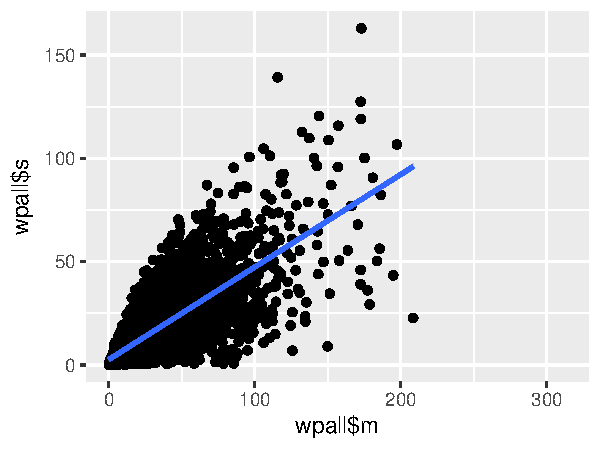
\includegraphics[width=\maxwidth]{figure/wp-1} 
\begin{kframe}\begin{alltt}
\hlkwd{qplot}\hlstd{(}\hlkwc{x}\hlstd{=wpall}\hlopt{$}\hlstd{ml,}\hlkwc{y}\hlstd{=wpall}\hlopt{$}\hlstd{sl)}\hlopt{+} \hlkwd{geom_smooth}\hlstd{(}\hlkwc{method}\hlstd{=}\hlstr{"lm"}\hlstd{)}
\end{alltt}


{\ttfamily\noindent\color{warningcolor}{\#\# Warning: Removed 2135 rows containing non-finite values (stat\_smooth).}}

{\ttfamily\noindent\color{warningcolor}{\#\# Warning: Removed 2135 rows containing missing values (geom\_point).}}\end{kframe}
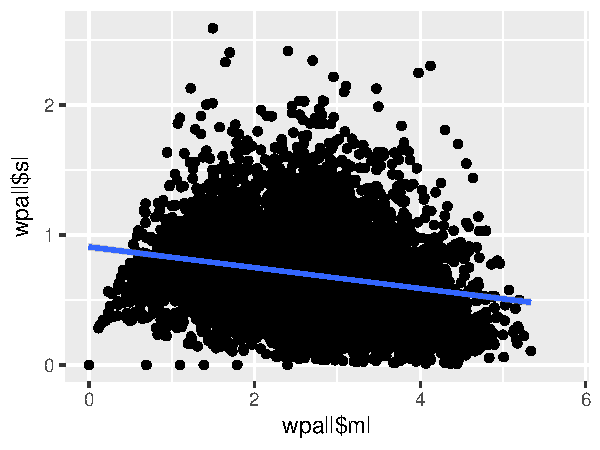
\includegraphics[width=\maxwidth]{figure/wp-2} 

\end{knitrout}

\begin{knitrout}
\definecolor{shadecolor}{rgb}{0.969, 0.969, 0.969}\color{fgcolor}\begin{kframe}
\begin{alltt}
\hlstd{nhanes}\hlopt{$}\hlstd{bmigroup} \hlkwb{<-} \hlnum{1}
\hlstd{nhanes}\hlopt{$}\hlstd{bmigroup[nhanes}\hlopt{$}\hlstd{bmi} \hlopt{>=} \hlnum{18}\hlstd{]} \hlkwb{<-} \hlnum{2}
\hlstd{nhanes}\hlopt{$}\hlstd{bmigroup[nhanes}\hlopt{$}\hlstd{bmi} \hlopt{>=} \hlnum{25}\hlstd{]} \hlkwb{<-} \hlnum{3}
\hlstd{nhanes}\hlopt{$}\hlstd{bmigroup[nhanes}\hlopt{$}\hlstd{bmi} \hlopt{>=} \hlnum{30}\hlstd{]} \hlkwb{<-} \hlnum{4}
\hlstd{nhanes}\hlopt{$}\hlstd{bmigroup[nhanes}\hlopt{$}\hlstd{bmi} \hlopt{>=} \hlnum{35}\hlstd{]} \hlkwb{<-} \hlnum{5}

\hlstd{nhanes}\hlopt{$}\hlstd{agegroup} \hlkwb{<-} \hlnum{1}
\hlstd{nhanes}\hlopt{$}\hlstd{agegroup[nhanes}\hlopt{$}\hlstd{age} \hlopt{>=} \hlnum{25}\hlstd{]} \hlkwb{<-} \hlnum{2}
\hlstd{nhanes}\hlopt{$}\hlstd{agegroup[nhanes}\hlopt{$}\hlstd{age} \hlopt{>=} \hlnum{35}\hlstd{]} \hlkwb{<-} \hlnum{3}
\hlstd{nhanes}\hlopt{$}\hlstd{agegroup[nhanes}\hlopt{$}\hlstd{age} \hlopt{>=} \hlnum{45}\hlstd{]} \hlkwb{<-} \hlnum{4}
\hlstd{nhanes}\hlopt{$}\hlstd{agegroup[nhanes}\hlopt{$}\hlstd{age} \hlopt{>=} \hlnum{55}\hlstd{]} \hlkwb{<-} \hlnum{5}
\hlstd{nhanes}\hlopt{$}\hlstd{agegroup[nhanes}\hlopt{$}\hlstd{age} \hlopt{>=} \hlnum{65}\hlstd{]} \hlkwb{<-} \hlnum{6}

\hlstd{nhanes} \hlopt \hlkwd{group_by}\hlstd{(sex)} \hlopt \hlkwd{summarise}\hlstd{(}\hlkwd{mean}\hlstd{(wearmin),}\hlkwd{sd}\hlstd{(wearmin)}\hlopt{/}\hlkwd{sqrt}\hlstd{(}\hlkwd{length}\hlstd{(wearmin)))}
\end{alltt}
\begin{verbatim}
## # A tibble: 2 � 3
##     sex `mean(wearmin)` `sd(wearmin)/sqrt(length(wearmin))`
##   <int>           <dbl>                               <dbl>
## 1     1        862.4040                           1.0745519
## 2     2        839.2255                           0.9610608
\end{verbatim}
\begin{alltt}
\hlstd{nhanes} \hlopt \hlkwd{group_by}\hlstd{(race)} \hlopt \hlkwd{summarise}\hlstd{(}\hlkwd{mean}\hlstd{(wearmin),}\hlkwd{sd}\hlstd{(wearmin)}\hlopt{/}\hlkwd{sqrt}\hlstd{(}\hlkwd{length}\hlstd{(wearmin)))}
\end{alltt}
\begin{verbatim}
## # A tibble: 5 � 3
##    race `mean(wearmin)` `sd(wearmin)/sqrt(length(wearmin))`
##   <int>           <dbl>                               <dbl>
## 1     1        838.3973                            1.504752
## 2     2        837.8630                            4.226087
## 3     3        848.6774                            0.944356
## 4     4        868.9508                            1.864345
## 5     5        855.5710                            3.544238
\end{verbatim}
\begin{alltt}
\hlstd{nhanes} \hlopt \hlkwd{group_by}\hlstd{(bmigroup)} \hlopt \hlkwd{summarise}\hlstd{(}\hlkwd{mean}\hlstd{(wearmin),}\hlkwd{sd}\hlstd{(wearmin)}\hlopt{/}\hlkwd{sqrt}\hlstd{(}\hlkwd{length}\hlstd{(wearmin)))}
\end{alltt}
\begin{verbatim}
## # A tibble: 5 � 3
##   bmigroup `mean(wearmin)` `sd(wearmin)/sqrt(length(wearmin))`
##      <dbl>           <dbl>                               <dbl>
## 1        1        853.8333                            7.185609
## 2        2        851.4379                            1.257627
## 3        3        855.4751                            1.212399
## 4        4        847.2281                            1.658649
## 5        5        839.8965                            2.096613
\end{verbatim}
\begin{alltt}
\hlstd{nhanes} \hlopt \hlkwd{group_by}\hlstd{(agegroup)} \hlopt \hlkwd{summarise}\hlstd{(}\hlkwd{mean}\hlstd{(wearmin),}\hlkwd{sd}\hlstd{(wearmin)}\hlopt{/}\hlkwd{sqrt}\hlstd{(}\hlkwd{length}\hlstd{(wearmin)))}
\end{alltt}
\begin{verbatim}
## # A tibble: 6 � 3
##   agegroup `mean(wearmin)` `sd(wearmin)/sqrt(length(wearmin))`
##      <dbl>           <dbl>                               <dbl>
## 1        1        841.3575                            2.053093
## 2        2        845.0387                            1.823399
## 3        3        856.7826                            1.809899
## 4        4        876.1550                            1.893967
## 5        5        853.2721                            1.875862
## 6        6        839.1086                            1.365020
\end{verbatim}
\begin{alltt}
\hlcom{#nhanes %>% group_by(sex,race,bmigroup) %>% summarise(mean(wearmin),sd(wearmin)/sqrt(length(wearmin)))}


\hlkwd{qplot}\hlstd{(}\hlkwc{x}\hlstd{=wearmin,}\hlkwc{y}\hlstd{=modvigmin,}\hlkwc{data}\hlstd{=nhanes)}
\end{alltt}
\end{kframe}
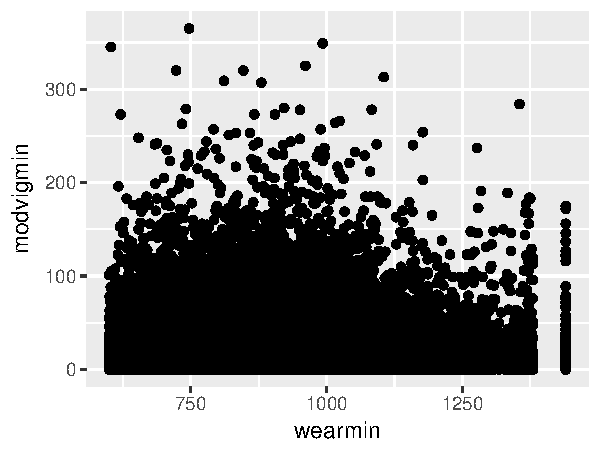
\includegraphics[width=\maxwidth]{figure/wp2-1} 
\begin{kframe}\begin{alltt}
\hlkwd{qplot}\hlstd{(}\hlkwc{x}\hlstd{=wearmin,}\hlkwc{y}\hlstd{=lightmin,}\hlkwc{data}\hlstd{=nhanes)}
\end{alltt}
\end{kframe}
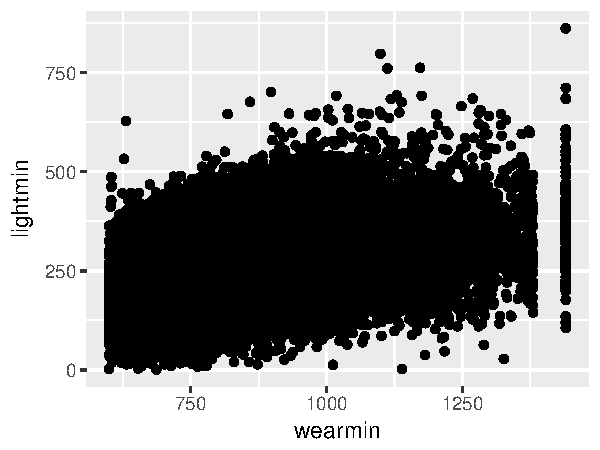
\includegraphics[width=\maxwidth]{figure/wp2-2} 

\end{knitrout}


\end{document}
